\chapter{Misinformation Spread on Networks}\label{ch:misinfo}

\section{Introduction}

\section{Literature Review\label{sec:liter}} 
 Recent literature has explored strategic models to study the spread of misinformation in networks~\cite{sikder2020minimalistic, acemoglu2021model, jackson2022learning,mostagir2023social,bloch2018rumors, kranton2024social}. The ones closest to our work include~\cite{jackson2022learning, acemoglu2021model}. In particular,~\cite{acemoglu2021model} presents a model of agents homogeneous in prior beliefs and preferences to study the extent of misinformation in networks. We consider heterogeneity in agent preferences. In~\cite{jackson2022learning} content is shared but it mutates in each exchange and users observing the history of spread seek to learn about the veracity of the mutated content. In our work, users' prior beliefs are a product of differing spread dynamics for true and false content and posterior beliefs are updated using user's private signals. Thus our model allows us to capture the information aggregation and peer filtering phenomenon absent in earlier work.
Other recent work explores how groups learn in networks about the state of the world.~\cite{huang2024learning} studied a setting where users repeatedly and strategically share information with their peers about the state of the world. They studied how the speed of learning is affected by the network structure.~\cite{dasaratha2019aggregative} studied study a setting where agents express how likely it is that a particular piece of content is true based on a private signal and actions of their neighbors. They showed that there was a confounding effect where one agent can have an outsized impact on another by influencing multiple peers. Like our model, these works consider Bayesian agents taking sequential actions in a social network but unlike our model they consider homogeneous user populations and do not make use of heterogeneous agents with differing types and  behaviors.  

~\cite{mostagir2022learning} studied a setting more similar to ours in that it considers heterogeneous agents for whom both the alignment and veracity matter. In their model, there exists both simple and sophisticated typed agents and they examine the contexts in which one type outperforms the other in learning. An important distinction between all of these works and ours is for the above works agents are learning from a local context, the actions of their neighbors, whereas agents in our model use global information about the average veracity of the content.~\cite{kranton2024social}studies a two stage information sharing setting where a seller chooses to share high or low quality information about its product and consumers then choose to share this information with their peers. The consumers decide to share after forming a belief about the quality given the information from the seller. Like in our work, the true quality of the information is hidden and consumers must make inferences. Unlike their model, we focus on the content sharing game among users within the network and our network equilibria focus on the global spread of different veracity of content. This work explores the phenomenon of peer filtering and the ability of the network as a whole to filter out more false content than true content thus leading to a higher average veracity of true content in the network as compared to content outside the network.

\section{Model}
We introduce a model for users interacting on an online platform. At a high level, users are shown content and must choose to share or not share that content. Content that is shared is shown to more users who will then face the same decision themselves. We assume that the sharing decisions between users are independent. We now describe the features of the content and the users that will factor into determining if a user shares or not. 
\textbf{Content Features} We assume that content has some veracity; either true (\true) or false (\false) and the proportion of true content entering the network is $p$. In addition, content is either inclined left or right. 
\textbf{User Features} Users themselves also have a political inclination. What matters is that if a content-user pair are aligned (\alg) or misaligned (\mal). A pair is aligned if they both share a left-leaning inclination or both share a right-leaning inclination. Otherwise they are misaligned. Users also care about the veracity of content. We assume that, keeping the alignment the same, that all users would at least weakly prefer to share content that is true. Likewise, we assume that keeping the veracity of content the same users would weakly prefer share content that is aligned with them. 

This leads us to develop a set of 4 different types of users. All users get positive utility for sharing content that is true and aligned and negative utility for sharing content that is misaligned and false. How they differ is their payouts for content that is aligned but false and misaligned but true. We define the four types of users as follows: 
\begin{itemize}
    \item \textbf{Impartial Truthtellers} (\IT) get positive utility from sharing news that is true irrespective of alignment. 
    \item \textbf{Impartial Fabulists} (\IF) get positive utility from sharing content that is true or aligned. 
    \item \textbf{Partisan Fabulists} (\PF) get positive utility from sharing content that is aligned. 
    \item \textbf{Partisan Truthtellers} (\PT) get positive utility from sharing content that is aligned and true. 
\end{itemize}


The action of not sharing is normalized to have a utility of 0. But what complicates matters is that while the users see the inclination of content they do directly observe the veracity of the content. Instead, when the ith user receives content $k$, she gets some signal $s_{ik} \in [0,1]$. True signals are distributed i.i.d. by some distribution $F^\true$ and false signals are distributed by some other distribution $F^\false$. We will use $f^\true$, and $f^\false$ to denote the probability density functions of $F^\true$ and  $F^\false$. We assume that $F^\true$ stochastically dominates $F^\false$ so that higher signals are more likely to be true than false.  Although we can generalize later, for now we will assume that the signals have a pdf of 
\[
f^\true(s) = 2s , f^\false = 2(1-s)
\]

In general, users are Bayesian agents with some prior $\delta$ belief about the veracity of content. Later, we will describe how this $\delta$ is endogenous to the model. Given a prior and a signal $s_{ik}$, a user's belief that a content is true, $\alpha_k$, follows from Bayes' Rule. 
\begin{equation}
    \Pr(\alpha_k = \true | s_{ik} = x ) = \frac{\delta x}{ \delta x + (1-\delta) (1-x) }\defeq \hat{\delta}(x)
\end{equation}

Following this rule, we know that if the user has a prior of $50\%$, they think content is equally likely to be true or false, then their posterior belief is exactly the signal they received. 
\section{Single User Behavior}

Each user receives a piece of content, consumes it for a signal, and must make a determination on whether to share it or not. A user will share content exactly if their expected utility is positive and not share otherwise.  We normalize the utility of sharing positive utility content to be $+1$ and the utility of sharing negative utility content to be $-1$. Therefore the expected utility of sharing for each type receiving a signal $x$ is characterized by 
\begin{tabular}{|c|c|c|c|c|}
   \hline 
   &  \IT & \PT & \IF & \PF \\
   \hline 
  \alg & $2\hat{\delta} -1$ & $2\hat{\delta} -1$ & $1$ & $1$ \\
  \mal & $2\hat{\delta} -1$ & $-1$ & $2\hat{\delta} -1$ & $-1$ \\
  \hline 
\end{tabular}

Notice however that who shares content when $2\hat{\delta} -1 > 0$ shares if and only if $x > 1 - \delta$. 

We can apply this characterization of the probabilities at which a user shares aligned or misaligned content to state the probability with which a user shares content of a given alignment and veracity. We use ${\beta(\delta)}^\alpha_{a,t}$ to be this probability that a with with type t and alignment $a$ shares content with veracity $\alpha$.  It is characterized by 
\begin{equation}
    {\beta(\delta)}^\alpha_{a,t} = \begin{cases} 1  & \text{ if t=\IF or \PF and } a=\alg \\
    0 & \text{if t=\PT or t=\PF and } a=\mal \\ 
    ?? & \text{Else} \end{cases}
\end{equation}


Given this sharing behavior across types and the type information of the network we can state the probablity that a user chosen uniformly at random shares true or false content. 
\begin{equation}\label{eq:share-probabilities}
\beta^\alpha(\delta) \defeq \sum_{a \in \{\alg, \mal\}} \frac{1}{2} \cdot \sum_{t \in \Theta}  \theta_t  \beta^\alpha_{a, t} = \frac{1}{2} \left(1 - \tt + (\tt+\tm) \overline{\mathrm{F}}_\alpha(1-\delta)  \right), 
\end{equation}

Finally, we state the result that for all prior beliefs $\delta$,  true content is preferred over false. 


\section{Spread Dynamics}
To analyze the spread dynamics in the network, suppose users in the network share a content of veracity $\alpha$ with fixed probability $\beta^\alpha$. Given the preceding analysis of a single user's behavior, we assume that $\beta^\true \geq \beta^\false$. Next, suppose a content with veracity $\alpha$ is introduced at time $0$ in the network. The number of users $X^{\alpha}(\tau)$ that see the content for the first time at time $\tau$ is random and depends on how many users choose to share the content at time $\tau - 1$. We have $X^\alpha(0) = 1$, and given the assumptions on the spread dynamics, we have $X^\alpha(1) = \kappa$ if the user chooses to share the content, otherwise $X^\alpha(1) = 0$. In general, we have 
\begin{align} \label{eq:branching_process}
    X^{\alpha}(\tau + 1) =\sum_{i= 1}^{X^{\alpha}(\tau)} {\kappa \cdot Z_i}
\end{align} 
where $Z_i$ is the indicator variable which takes value $1$ if the $i^{th}$ user among the $X^{\alpha}(\tau)$ users exposed to the content at time $\tau$ chooses to share the content. The analysis of the single user behavior in the preceding section shows that $Z_i = 1$ with probability $\beta^{\alpha}$ for a randomly chosen user. Thus, we conclude that the conditional distribution of $X^{\alpha}(\tau + 1)$ given $X^{\alpha}(\tau)$ is $\kappa$ times a Binomial random variable with parameters $X^{\alpha}(\tau)$ and $\beta^{\alpha}$. Thus, $X^{\alpha}(\tau)$ follows a Galton-Watson branching proces%s~\cite{athreya2004branching}. 
Furthermore, the expected number of users who observe the content for the first time at time $\tau$ is given by $\ex{X^\alpha(\tau)} = (\kappa \beta^\alpha)^\tau$. As we describe below, the dynamics of this process is captured by $\kappa\beta^{\alpha}$, called its {\em branching rate}.


If the branching rate $\kappa \beta^\alpha$ is strictly less than $1$, the process eventually equals zero, meaning that the users eventually stop sharing the content. In this case, the total expected number of users who see the content is finite, and is given by
% \begin{flalign}\label{eq:expected_spread}
% \sum_{\tau =0}^\infty (\kappa \beta^\alpha)^\tau = \frac{1}{1-\kappa \beta^\alpha}. &&
% \end{flalign}
\begin{align}\label{eq:expected_spread}
\sum_{\tau =0}^\infty (\kappa \beta^\alpha)^\tau = \frac{1}{1-\kappa \beta^\alpha}. &&
\end{align}
On the other hand, if the branching rate is strictly greater than $1$, then with positive probability the process never equals zero, implying that the content is shared throughout the network, i.e., the content goes ``viral''. The probability $q^\alpha$ with which the content goes viral is obtained as the largest solution in $[0,1]$ to the following extinction equation:
\begin{align} \label{eq:viral-prob}
    1- q^{\alpha} = 1-\beta^{\alpha} + \beta^{\alpha}(1 - q^{\alpha})^{\kappa}. &&
\end{align}
To interpret the equation, the left-hand side denotes the probability that the content does not go viral. This can only happen if (1) either the first user decides not the share the content (which happens with probability $1-\beta^\alpha$) or (2) the first user shares the content (an event with probability $\beta^\alpha$) but none of the $\kappa$ subprocesses originating from the $\kappa$ peers to whom the content is shared go viral (which occurs with probability $(1-q^\alpha)^\kappa$).

\begin{figure}
 \centering
\begin{subfigure}{0.25\textwidth}
    \includegraphics[width=\textwidth]{Figures/bust.pdf}
    \caption{}
\end{subfigure}%
\hspace{0.10\textwidth}%
\begin{subfigure}{0.25\textwidth}
 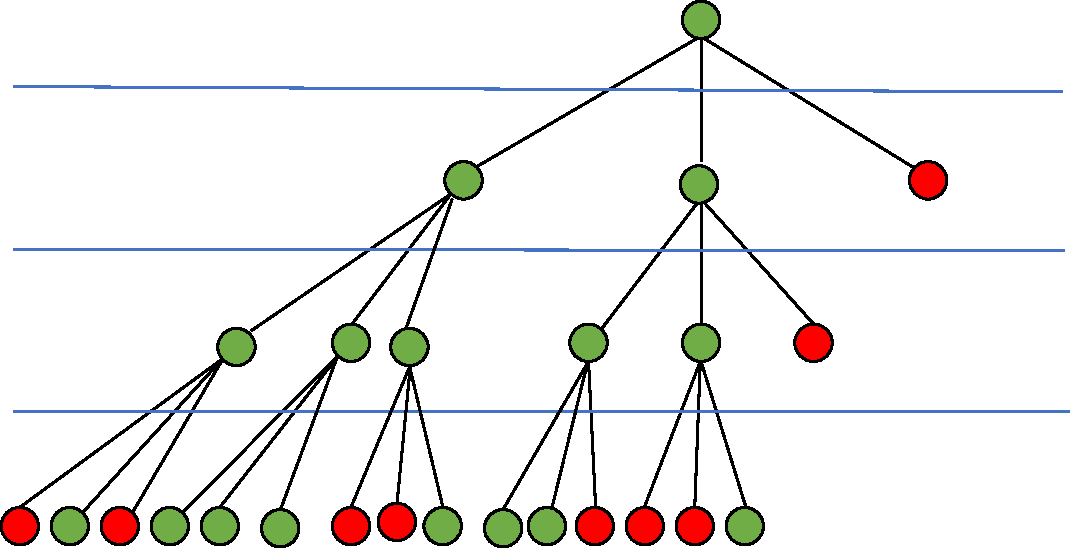
\includegraphics[width=\textwidth]{Figures/network_spread.pdf}
 \caption{}
\end{subfigure}
\caption{Spread of content in a large network, green nodes decide to share the content; red nodes decide not to share the content; (a) false content is less likely to be shared and the spread may go bust (b) true content is slightly more likely to be shared and may end up going viral.}\label{fig:spread-dynamics}

\end{figure}

When the effective branching factor is less than one, almost surely the spread will go extinct or ``bust''. Instead the expected number of users who see a particular piece of content is given by 
\begin{equation}
    \sum_{\ell=0}^\infty  {\left(\branch\right)}^\ell = \frac{1}{1-\branch }
\end{equation}
When it is greater than one however the content may not go extinct. In this context we may say that content goes ``viral''. This occurs with some positive probability, $q^\alpha$ defined by: 
\begin{equation*}
    1-q^\alpha = 1 -\beta^\alpha + \beta^\alpha \left( \sum_{\ell=0}^\infty \pi_\ell {\left(1-q^\alpha\right)}^\ell \right)
\end{equation*}

To interpret this equation as tracking how content could go extinct in two different ways. The first is $1-q^\alpha$, this is definitionally the probability content doesn't go viral. On the right-hand side, we observe content doesn't go viral if it is not shared by the first user, $1-\beta^\alpha$, or it is shared but each descendant branch goes extinct, $\beta^\alpha \left( \sum_{\ell=0}^\infty \pi_\ell {\left(1-q^\alpha\right)}^\ell \right)$.

Applying this logic, we characterize the expected proportion of true content a user actually sees. We assign $\Theta$ to represent this quantity. We separate this into three cases. 
\textbf{Case 1}: $\branch{\true} \leq \branch{\false} \leq 1 $ 
In this case, both the spread true and false news die out after a finite number of rounds. The amount of true content a user sees in the network depends on the relative size of the expected trees for true and false content weighted by how frequent each appears. That is 
\[ \Theta = \frac{ \frac{p}{ 1 - \branch{\true}}}{ \frac{p}{1-\branch{true}} + \frac{1-p}{1-\branch{\false}}} \]


\textbf{Case 2}:  $\branch[\true] \geq  1 \geq \branch{\false} \leq 1 $ 
In this case just the true content can go viral. Therefore, the true news dominates and $\theta=1$. This situation is achievable by the correct setting parameters would be ideal for society. 

\textbf{Case 3}:  $\branch[\true] >\branch{\false} >  1 $ 
In this case both true and false content sometimes goes viral. What matters then is their respective probabalities of virality how much true and false content a user observes. That is 
\begin{equation}
    \theta = \frac{pq^\true}{pq^\true + (1-p)q^\false } 
\end{equation}


\subsection{Equibriums} 

At the beginning of the model, we assumed that users' prior belief $\delta$ was fixed. Now we will discuss how it is endogenous to the model. But in practice, their belief of the average veracity of the system should equal the proportion of true content actually in the network. If $\delta $ is such that $\delta = \Theta$ we call such a state an equilibrium. We designate equilibrium into three cases based on cases above. When both true and false content go extinct (case 1) we say we have a bust equilibrium. When true content goes viral but false goes extinct (case 2) we say we have a boom-bust equilibrium. Finally, when both true and false content goes viral (case 3) we say we are in a boom equilibrium.  We will now focus on properties of equilbria. 

The first property is the non-existence of the boom-bust equilbria. 
\begin{theorem}
    Every equilbrium of the network is either a boom equilibrium or a bust equilibrium. In particular, the network never admits a boom-bust equilibrium. 
\end{theorem}
\begin{proof}
    We proceed by proof by contradiction. Suppose that we have an equilibrium where $\branch{\true} > 1 > \branch{false}$ then only true content goes viral and $\Theta=1$. Since we have an equilibrium $\Theta = \delta = 1$. But applying this to equation $\ref{eq:share-probabilities}$ we find that $\beta^\true = \beta^\false$ which contradicts $\branch{\true} >\branch{false}$. 
\end{proof}

\begin{figure}
    \centering
  \scalebox{0.8}{  \begin{tikzpicture}[
    node distance=2cm,
    every node/.style={rounded rectangle, fill=blue!20, align=center, minimum width=3cm, minimum height=1.2cm},
    every path/.style={very thick, -{Latex[bend]}, draw=black},
    every label/.style={fill=white, inner sep=1pt}
]
% Node definitions
\node (prior) {prior belief $\delta$};
\node[above = of prior] (posterior) {posterior belief};
\node[right = of posterior] (sharing) {Sharing probabilities\\ $\beta^\true, \beta^\false$};
\node[below = of sharing] (proportion) {Proportion of true content\\ in the network $\Phi(\beta^\true, \beta^\false)$};
\node[fill=red!10] (equilibrium) at ($(posterior)!0.5!(proportion)$)  {Equilibrium: \\ $\delta = \Phi(\beta^\true(\delta), \beta^\false(\delta))$};

% Path definitions
\draw (prior) edge[bend left=25] node[midway, left, fill=none, xshift=0.4cm] {signal from\\ content\\ consumption} (posterior);
\draw (posterior) edge[bend left=45] node[midway, above, fill=none, yshift=-0.15cm] {single user\\ behavior} (sharing);
\draw (sharing) edge[bend left=25] node[midway, right,  fill=none, xshift=-0.65cm] {spread\\ dynamics} (proportion);
\draw (proportion) edge[bend left=45] node[midway, below, fill=none, yshift=0.15cm] {consistency\\ of beliefs} (prior);

\end{tikzpicture}}
\caption{Equilibrium in the network. Here $\beta^\true, \beta^\false$ are obtained from $\delta$ through~\eqref{eq:share-probabilities}, and the proportion of true content $\Phi(\beta^\true, \beta^\false)$ is given by~\eqref{eq:proportion-true}. An equilibrium corresponds to a value of $\delta$ for which the belief is consistent with spread dynamics.}\label{fig:equilibrium-fixed-point}

\end{figure}


Next, our next result is that for any equilibrium the equilibrium $\delta$ is lower bounded by the incoming veracity of content. 
\begin{theorem}
    In any equilibrium $\delta \geq p$
\end{theorem}

Equality can be realized in a system where all users are partisan fabulists ($\theta_{PF} = 1$). This is because all users are agnostic about the veracity of content, they only care about the alignment. We think of how much more $\delta$ is that $p$ as through the lens of the network and the sharing decisions of users as a filtering mechanism of content. When much more true content is seen by users, we say that the network is an effective filter. The reason that peers can act as a filter on veracity is that all types at least weakly care prefer true content over false hence true content is more likely to be shared and seen by more users.  Later in this work, we will discuss what properties of the network promote more effective peer filtering with an eye towards how a platform could promote networks that have greater peer-filtering effectiveness. First however, we discuss the properties of the other two type of equilibria. 

This Theorem states first that the condition for a boom equilibrium to exist is only that the expected number of shares is above or below a threshold dependent on the types in the system. Notice furthermore, that $\tm \in [0,1]$ so a boom equilibrium always exists if $\ex{\kappa} > 2$. The other thing this theorem states is the conditions for a bust equilibrium to exist. In essence, it depends on the relationship between $\ex{\kappa}$ and two curves, $\frac{2}{2+\tm}$ and $\kappa(\frac{p}{1-p})$. If $\ex{\kappa} $ then $\frac{2}{2+\tm}$, there is a unique bust equilbrium. This is exactly the case there there is no boom equilibrium. When $\ex{\kappa}$ is between the two curves there is one unique bust equilibrium and a boom equilibrium. When $\ex{\kappa}$ is above the curve $\kappa(\frac{p}{1-p})$ then there is only boom equilibria. Finally, if $\ex{\kappa}$ is exactly  on the curve $\kappa(\frac{p}{1-p})$ and if in addition $\frac{p}{1-p} < \frac{1}{2}$ there are exactly two bust equilibrium. This second condition is saying that there is more than twice as much false content than true. Having more false content in the system drives down beliefs and makes it easier for content to go bust. 
\begin{theorem}\label{thm:equilibria-existence}
    There exists a  boom equilibrium if and only if $\kappa >  \frac{2}{1+\tm}$. On the other hand, there exists a bust equilibrium if any of the following conditions are met: 
    \begin{itemize}
        \item $\kappa < \frac{2}{1+\tm}$ (a unique bust equilibrium exists); 
        \item $\kappa = \frac{2}{1+\tm}$ and $\gamma < \frac{1}{2}$ (a unique bust equilibrium exists);  
        \item If $\kappa \in \left(\frac{2}{1+\tm} , \kappa(\gamma) \right)$ and $\gamma < \frac{1}{2}$ (two bust equilibria exist);
        \item If $\kappa = \kappa(\gamma)$ and $\gamma < \frac{1}{2}$ (a unique bust equilibrium exists),
    \end{itemize}
    where $\gamma \defeq \frac{p}{1-p}$. Otherwise, there exists no bust equilibrium. Here, \[\kappa(\gamma) \defeq \frac{2 (\gamma-1) (\gamma+1)^3}{\gamma^4 (\tm+1)+\gamma^3 (-6 \tm-8 \tt+2)+12 \gamma^2 (\tm+\tt)-2 \gamma (4 \tm+3 \tt+1)+\tt-1}.\]
\end{theorem}


\textit{Proof Idea:} The proof is delicate; in particular the existence of fixed points of the $\Pi(\delta)$ depends on the spread dynamics because of the expression for $\Phi(\beta^\false, \beta^\true)$ in~\eqref{eq:proportion-true}.  In particular, given the case-by-case definition, it is not immediately clear if the function $\Pi$ is continuous over the interval $[0,1]$. We consider cases based on $\kappa$ and in each establish the  continuity of $\Pi(\delta)$ as defined in Section~\ref{sec:spread-equilibrium}. We then show that there are some values of $\delta \in (0, 1) $ where $\Pi(\delta) < \delta$ and for other values of $\delta \in (0, 1) $ where $\Pi(\delta) > \delta$. The fixed point condition is then satisfied by the intermediate value theorem. We achieve this by performing a careful perturbative analysis to identify the effect of perturbing $\delta$ close to specific values where the definition of the function $\Phi$ changes from one case to another. We provide the full details in the Appendix.

Theorem~\ref{thm:equilibria-existence} is stated only in terms of $\tm$ and $\tt$. This implies that the full type distribution does not directly influence the equilibria structure. Instead, what determines this is only the marginal distributions of the populations inclination towards truth-telling and partisanship.  Below we formally state this is as a proposition. 

\begin{proposition}
     Let $\theta, \theta' \in \Theta$ be two type distributions satisfying $\theta_{\IF}' + \theta_{\IT}' = \theta_{\IF} + \theta_{\IT}$  and $\theta_{\IT}' + \theta_{\PT}' = \theta_{\IT} + \theta_{\PT}$. Then two user populations with type distributions $\theta$ and $\theta'$ have the same set of equilibria for any $p \in (0,1)$ and $\kappa > 0 $. 
\end{proposition}

This proposition implies that the effect of changing the population has on the set of equilibrium is determined by $\tm$ and $\tt$. This observation is utilized in the next section where we alter these marginal distributions as we showcase how the peer filtering effect changes as a function of the population's change in types.
\section{Peer Filtering}



Now that we have developed the techniques to characterize the equilibria, we focus on the outcomes of interest in equilibria and control techniques to help the social network choose the socially desirable equilibrium. We focus in particular on the power of peers in the social network to include their own information and judgment independently and prevent the spread of false information. Peer filtering is a self-correcting phenomenon that moderates the diffusion on misinformation in the social network through an intricate relationship between individual behavior of users and the diffusion dynamics of the social network.  Two effects determine this phenomenon. First, when the level of misinformation diffusion is high, then users are more skeptical about the veracity of the information in the network and less engaged with sharing information. This reduces the diffusion of all information but more so  for false information thus reducing the fraction of misinformation in the network that goes viral. Second, when the level of both true and false information is comparable in the social network, then the users weigh their private signal more when deciding about the veracity of information. This leads to more independent decision making by the users. Subsequently the wisdom of the crowds emerges and true content goes more viral than false content. 



% In this section, we investigate the effects of various parameters on the peer-effect phenomenon. To do this, we introduce various metrics of interest in the next subsection, followed by numerical results that study these metrics in equilibrium as we vary the model parameters. In the end, we study non-discriminatory controls that the platform can use to improve the equilibrium peer-filtering effect and mitigate the effects of false content sources, low signal quality of users\kicomment{What do we mean by this?}, and high fraction of fabulists in the user population. Non-discriminatory controls are those that do not target specific users or content. \kicomment{The preceding sentence should either come earlier (in the intro?) or deleted.}

% %When the level of misinformation in the network is low the users weigh their private information less and are more engaged in sharing the content. This allows false information to easily sneak in and go viral. 

\subsection{Metrics}
{\small 
\begin{figure}[htbp]
\centering
\begin{tabular}{ccc} 
  \toprule
 Quantity  & & Metric \\
 \midrule
 Peer filtering effectiveness &   & ${\delta}/{p}$ \\
  Sensitivity & & $1- q^\false$\\
 Specificity  & & $q^\true$\\
 Engagement level & & $\delta \beta^\true + (1-\delta) \beta^\false$\\
 Volume &  & $pq^\true + (1-p) q^\false$\\
  \bottomrule
\end{tabular}
\caption{Various quantities of interest and the corresponding equilibrium metrics in the model.}\label{table:metrics}


\end{figure} }
To understand the effect these controls have on the spread of true and false content, we  study the \emph{peer filtering effectiveness} (the ratio of true content in the system to incoming true content) as well as the \emph{sensitivity} (fraction of false content filtered out), \emph{specificity} (fraction of true content not filtered out) and \emph{misinformation  level}, i.e., the proportions of true and false content circulating in the network in equilibrium. We examine how the peer-filtering effect depends on the composition of different types of users, informativeness of private signals, average veracity of content, and the spread factor. Alongside the peer-filtering effectiveness, we also study the impact on the \emph{engagement level} (the frequency that content is shared with) and the \emph{volume} of content that goes viral. These metrics are defined in the table above. 


Our theoretical analysis shows that the entire network acts as a filter that selectively amplifies true content over false content among those that go viral. We  complement this theoretical analysis with a numerical investigation using various metrics of interest. The first metric of interest is the magnitude of the peer-filtering effect, which we capture using the metric of {\em peer-filtering effectivness}, defined as $\delta/p$. Observe that Theorem~\ref{thm:delta_geq_p} states that this metric is at least one; higher values of peer-filtering effectiveness suggests that the  relatively more of the false content is filtered out, i.e., the filtering effect is stronger, whereas values closer to one suggests a weak filtering effect. 

The next metrics of interest are the rates of false positives and false negatives due to the peer filtering, where positives correspond to content that do not go viral (i.e., the network effectively filters them out) and negatives correspond to content that go viral. We capture these rates using the standard notions of {\em sensitivity}, capturing the fraction of the false content that does not go viral, and {\em specificity}, capturing the fraction of true content that goes viral. By definition, we have the sensitivity equal to $1- q^\false$ and specificity equal to $q^\true$. 

Finally, we also study the effect of peer-filtering on metrics that are of interest to the network, namely the engagement level of the users (defined as the proportion of the content seen by a user that gets shared) and the volume (defined as the proportion of content that arrives to the network and goes viral). The definitions of the various metrics are summarized in Table~\ref{table:metrics}.


\subsection{Metrics}
%% uncomment this for wrap table
% {\small 
% \begin{wraptable}{r}{0.4\textwidth}
% \centering
% \begin{tabular}{ccc} 
%   \toprule
%  Quantity  & & Metric \\
%  \midrule
%  Peer filtering effectiveness &   & ${\delta}/{p}$ \\
%   Sensitivity & & $1- q^\false$\\
%  Specificity  & & $q^\true$\\
%  Engagement level & & $\delta \beta^\true + (1-\delta) \beta^\false$\\
%  Volume &  & $pq^\true + (1-p) q^\false$\\
%   \bottomrule
% \end{tabular}
% \caption{Various quantities of interest and the corresponding equilibrium metrics in the model.}\label{table:metrics}

% \end{wraptable} }

{\small 
\begin{figure}
\centering
\begin{tabular}{ccc} 
  \toprule
 Quantity  & & Metric \\
 \midrule
 Peer filtering effectiveness &   & ${\delta}/{p}$ \\
  Sensitivity & & $1- q^\false$\\
 Specificity  & & $q^\true$\\
 Engagement level & & $\delta \beta^\true + (1-\delta) \beta^\false$\\
 Volume &  & $pq^\true + (1-p) q^\false$\\
  \bottomrule
\end{tabular}
\caption{Various quantities of interest and the corresponding equilibrium metrics in the model.}\label{table:metrics}

\end{figure} }

{\small 
\begin{figure}
\centering
\scalebox{0.9}{
\begin{tabular}{cccccc} 
  \toprule
  Quantity & Peer filtering effectiveness & Sensitivity & Specificity & Engagement level & Volume \\
 \midrule
  Metric & ${\delta}/{p}$  & $1- q^\false$ & $q^\true$ & $\delta \beta^\true + (1-\delta) \beta^\false$ & $pq^\true + (1-p) q^\false$\\
  \bottomrule
\end{tabular}
}
\caption{Various quantities of interest and the corresponding equilibrium metrics in the model.}\label{table:metrics}

\end{figure}
}
To understand the effect these controls have on the spread of true and false content, we  study the \emph{peer filtering effectiveness} (the ratio of true content in the system to incoming true content) as well as the \emph{sensitivity} (fraction of false content filtered out), \emph{specificity} (fraction of true content not filtered out) and \emph{misinformation  level}, i.e., the proportions of true and false content circulating in the network in equilibrium. We examine how the peer-filtering effect depends on the composition of different types of users, informativeness of private signals, average veracity of content, and the spread factor. Alongside the peer-filtering effectiveness, we also study the impact to the \emph{engagement level} (the frequency that content is shared with) and the \emph{volume} of content that goes viral. These metrics are defined in the table above. 

\subsection{Results} 
% \begin{figure}
%         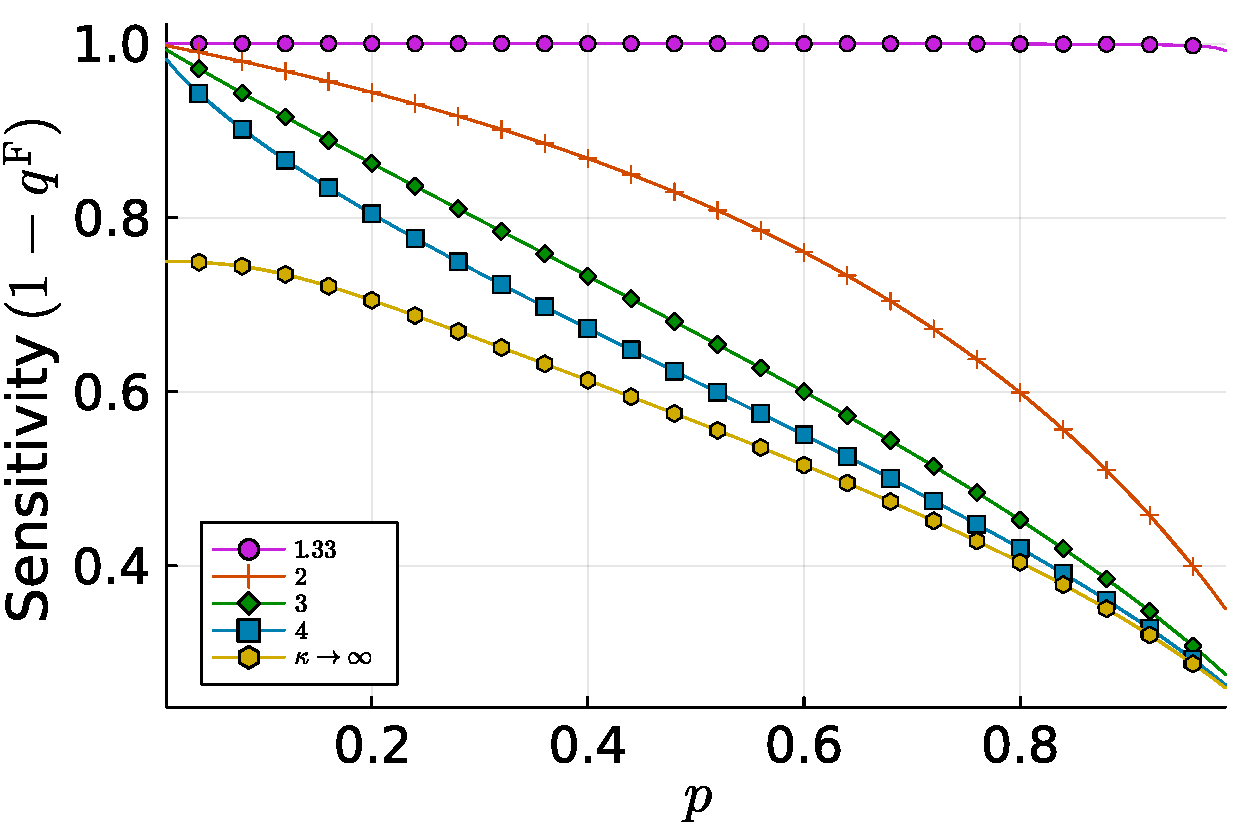
\includegraphics[width = \textwidth]{Figures/sensitive.pdf}
% \end{figure}\label{fig:sensitivity_specificity}

\begin{figure}
    \centering
    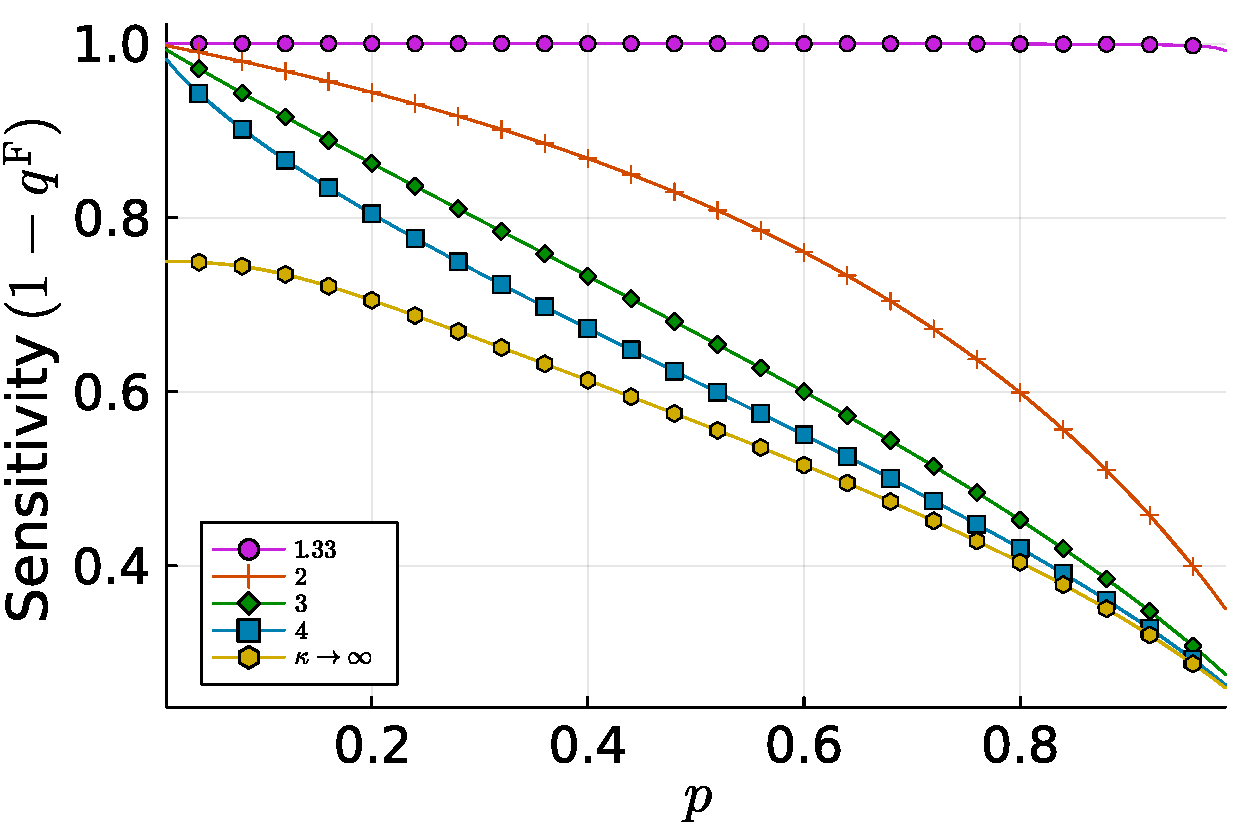
\includegraphics[width = 0.4\textwidth]{Figures/sensitive.pdf}
    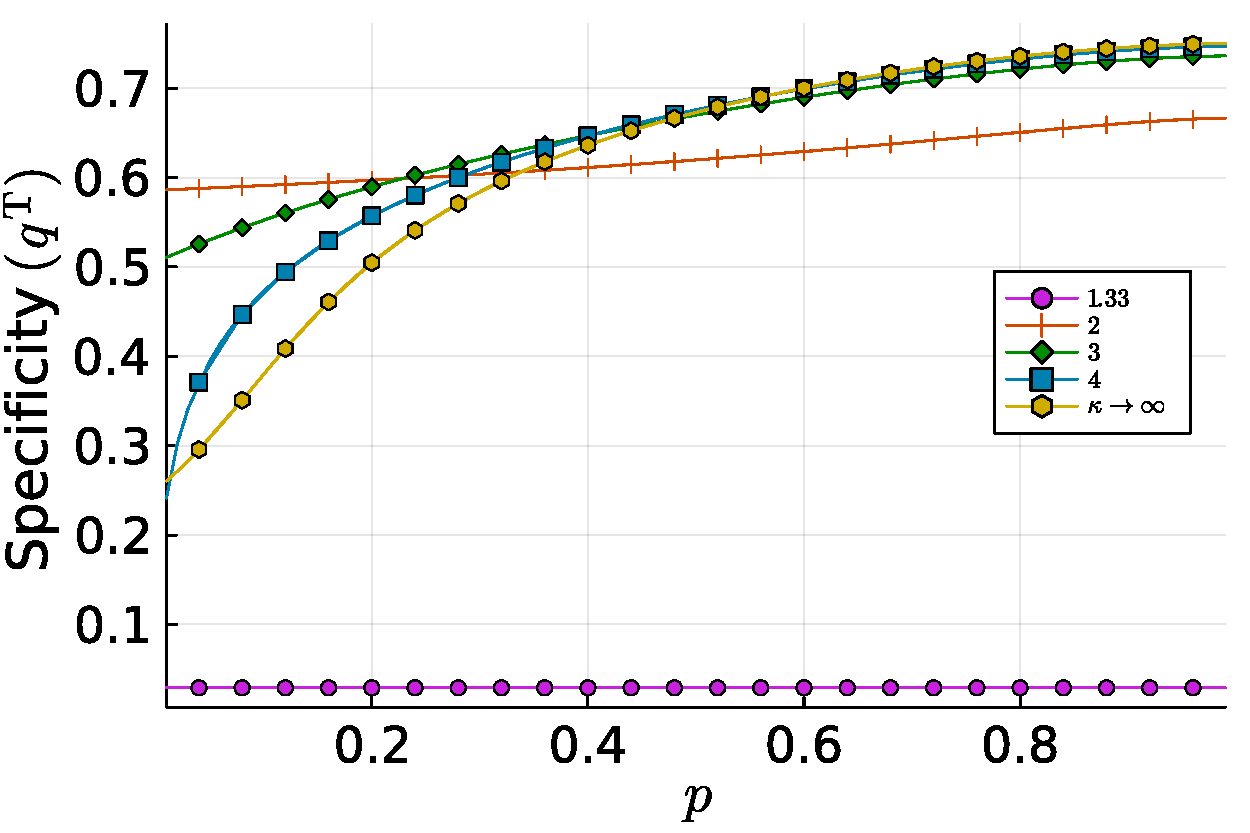
\includegraphics[width = 0.4\textwidth]{Figures/specit.pdf}
    \caption{(a) Sensitivity and (b) Specificity in the boom equilibrium as a function of the average veracity $p$ of new content for different values of $\kappa$.}\label{fig:sensitivity_specificity}
\end{figure}
We perform a numerical analysis on a population consisting of equal parts of all four types i.e., $\theta_{\IF} = \theta_{\PF} = \theta_{\IT} = \theta_{\PT} = 1/4$. We start with a discussion of the sensitivity and specificity as a function of $p$ and $\kappa$ and then we will look at how the engagement, volume, and equilibrium belief change.  


% \begin{figure}[htbp]
% \centering
%     \begin{tabular}{cc}
%     %\begin{tabular}
% 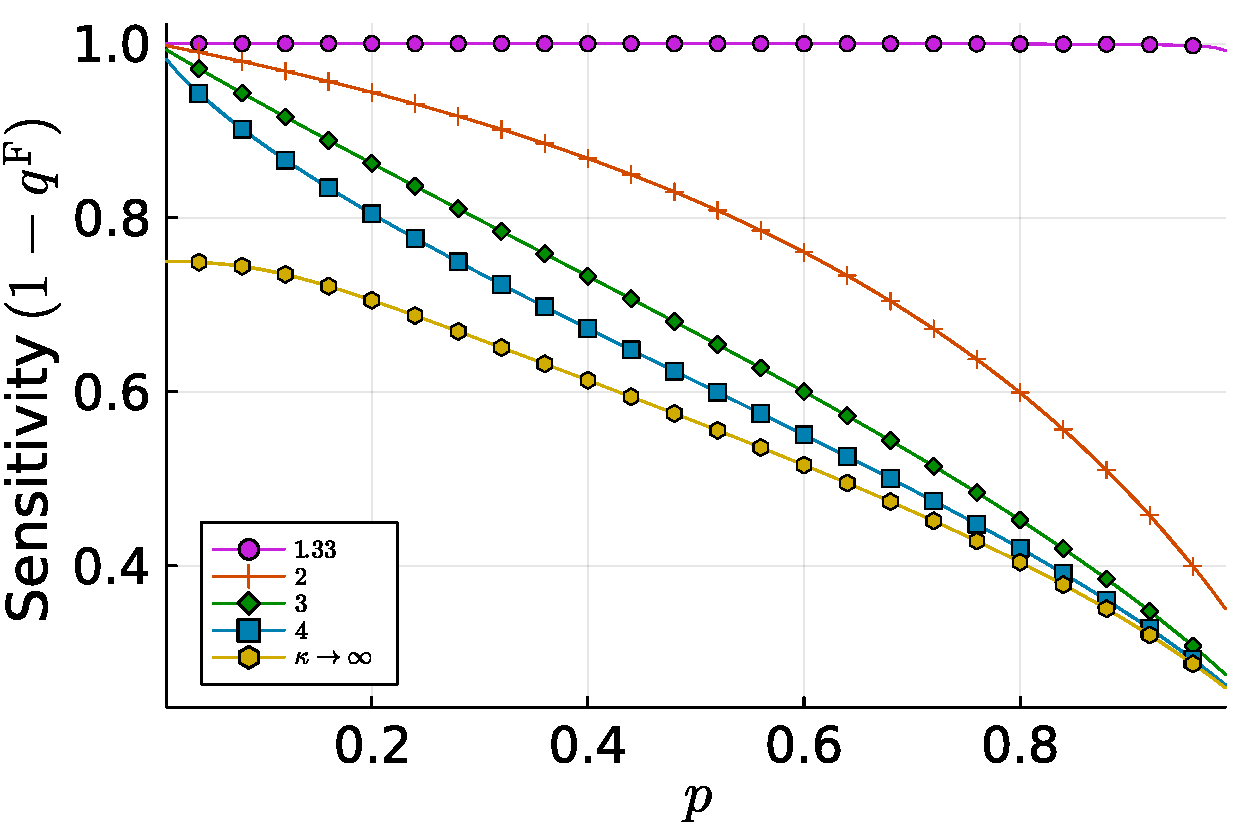
\includegraphics[width = 0.25\textwidth]{Figures/sensitive.pdf}
% 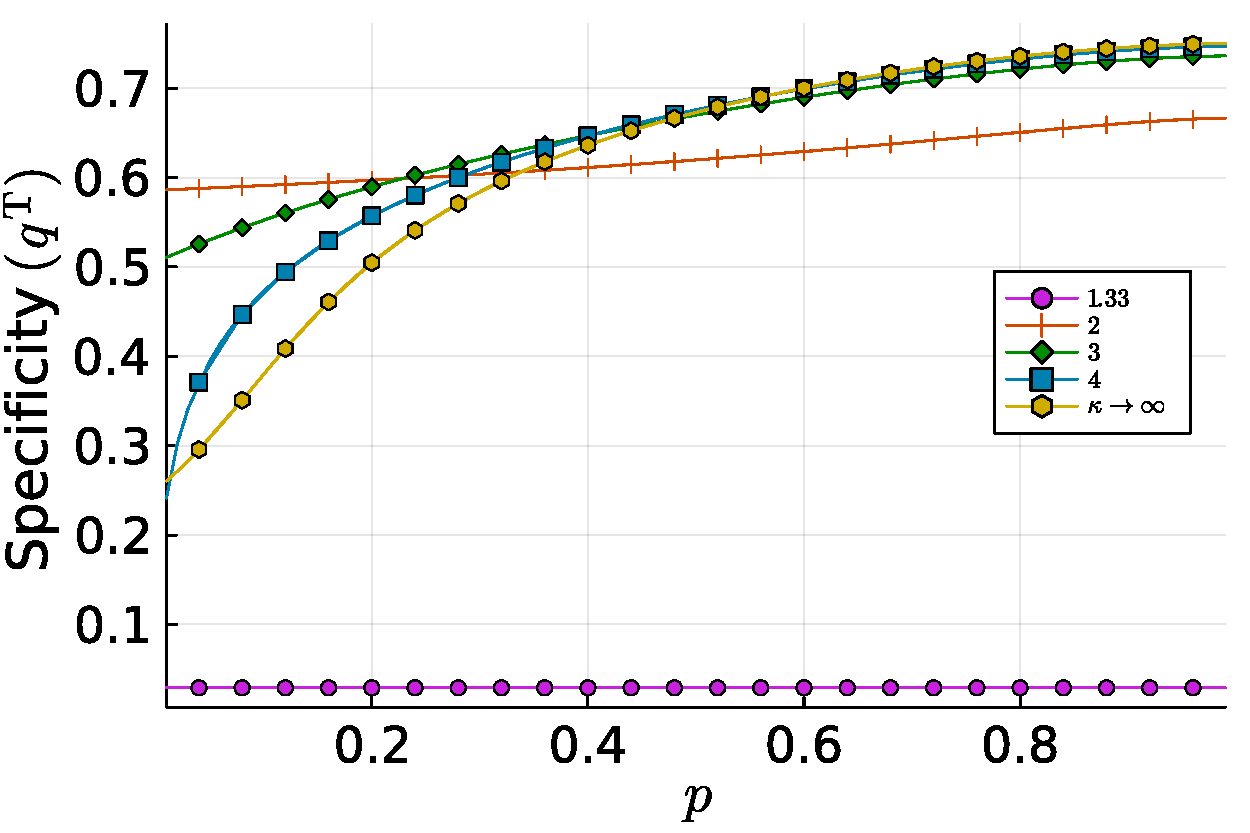
\includegraphics[width = 0.25\textwidth]{Figures/specit.pdf}
% \\{\small(a\right) \hspace{0.25\textwidth} {\small(b\right)
% \end{tabular}
% \caption\left(a) Sensitivity and (b) Specificity in the boom equilibrium as a function of the average veracity $p$ of new content for different values of $\kappa$.}\label{fig:sensitivity_specificity}
% \end{figure}

% \begin{wrapfigure}{R}{0.25\textwidth}
%     \centering
%     \begin{subfigure}{0.22\textwidth}
%         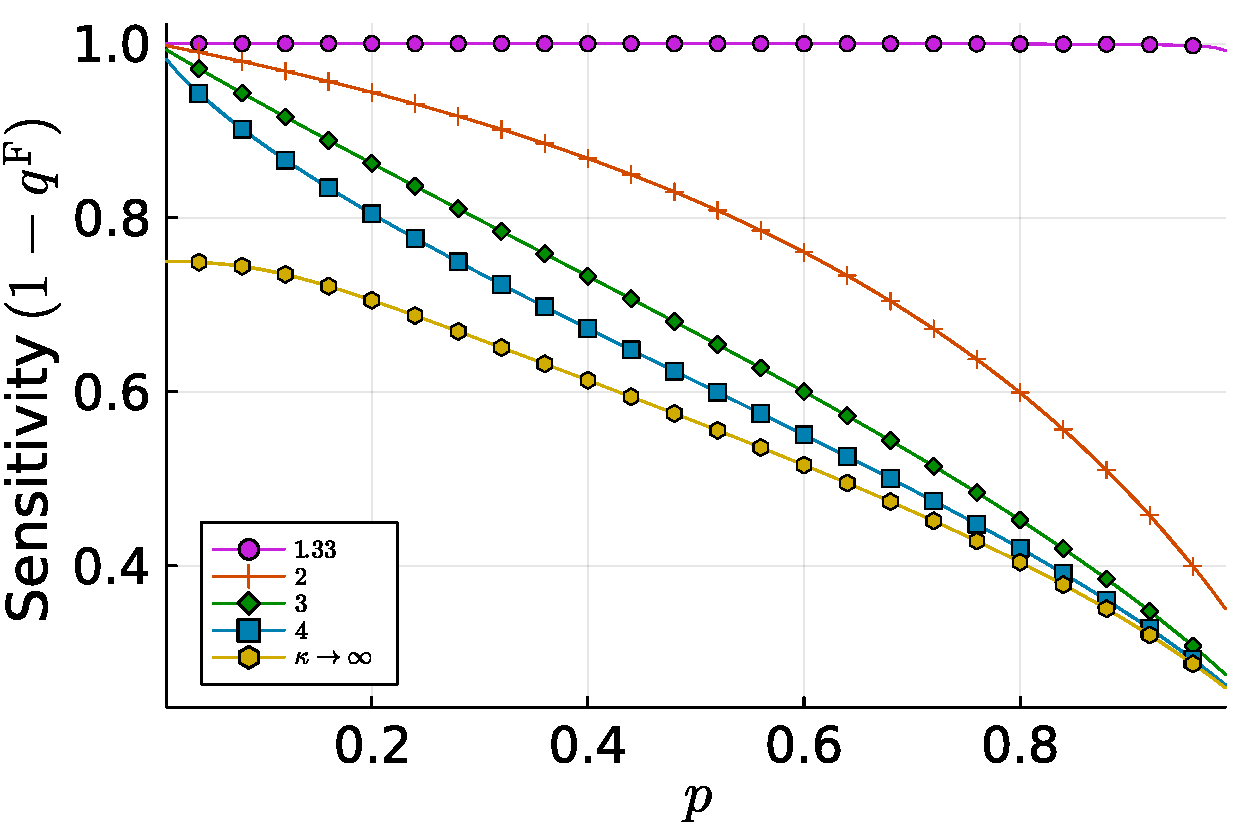
\includegraphics[width = \textwidth]{Figures/sensitive.pdf}
%         \caption{}
%     \end{subfigure}
%     \begin{subfigure}{0.22\textwidth}
%         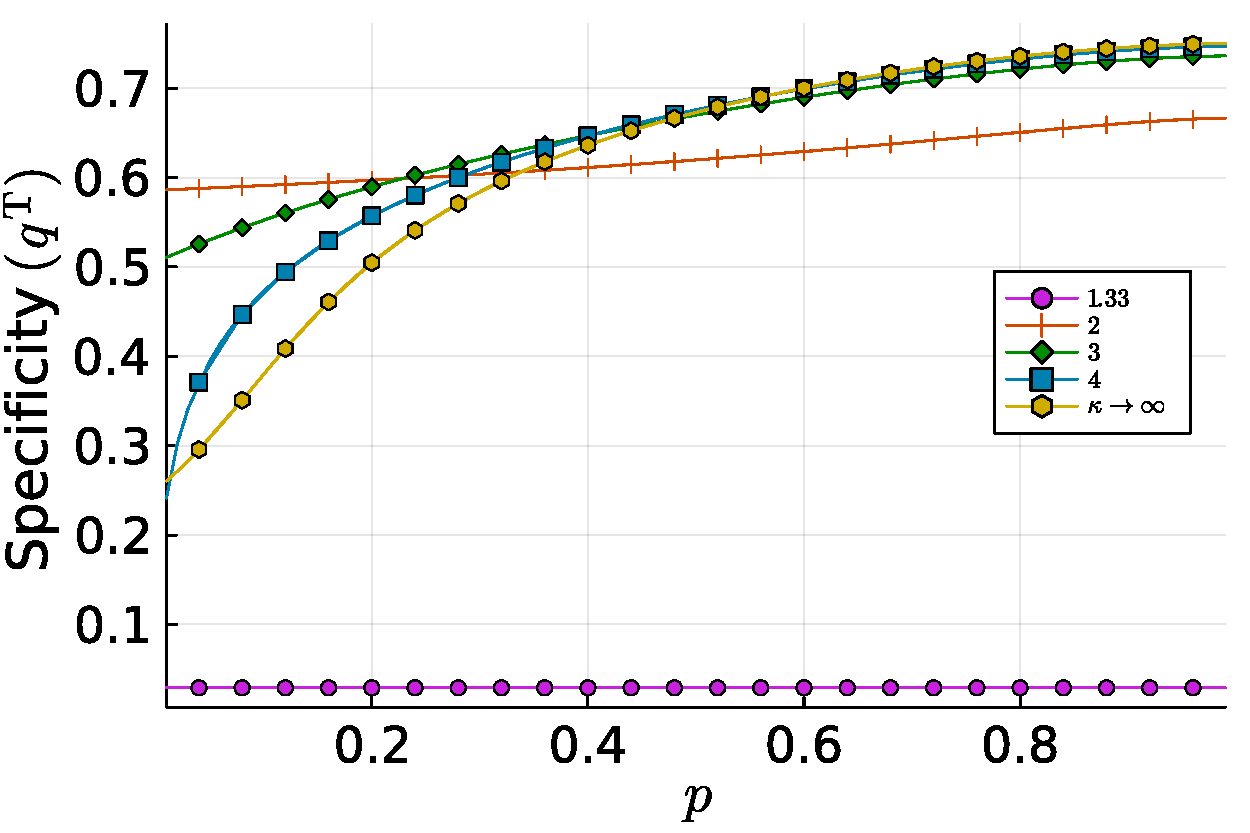
\includegraphics[width = \textwidth]{Figures/specit.pdf}
%         \caption{}
%     \end{subfigure}
% \caption\left(a) Sensitivity and (b) Specificity in the boom equilibrium as a function of the average veracity $p$ of new content for different values of $\kappa$.}\label{fig:sensitivity_specificity}
% \end{wrapfigure}

\subsubsection{Sensitivity and Specificity}
% \begin{figure}
%     \centering
%     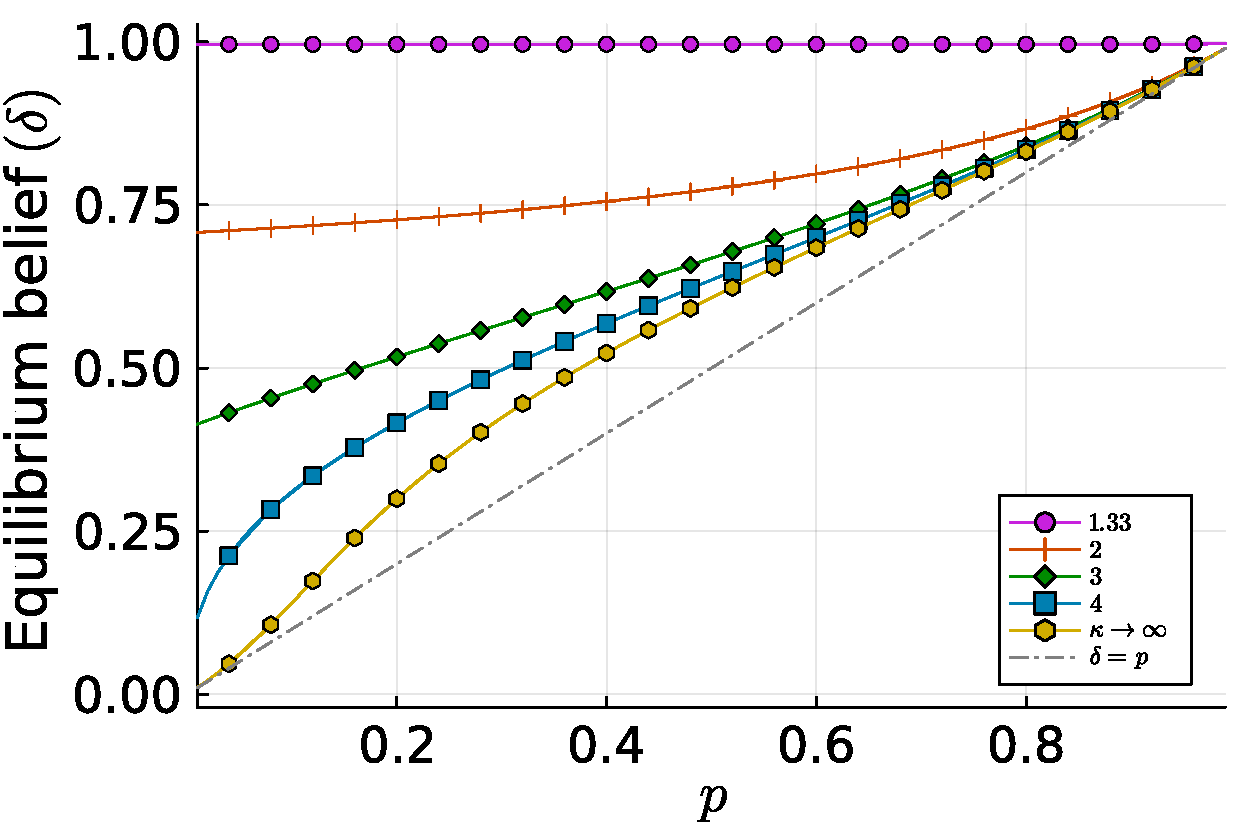
\includegraphics[width=0.22\linewidth]{Figures/p_vs_delta.pdf}
%     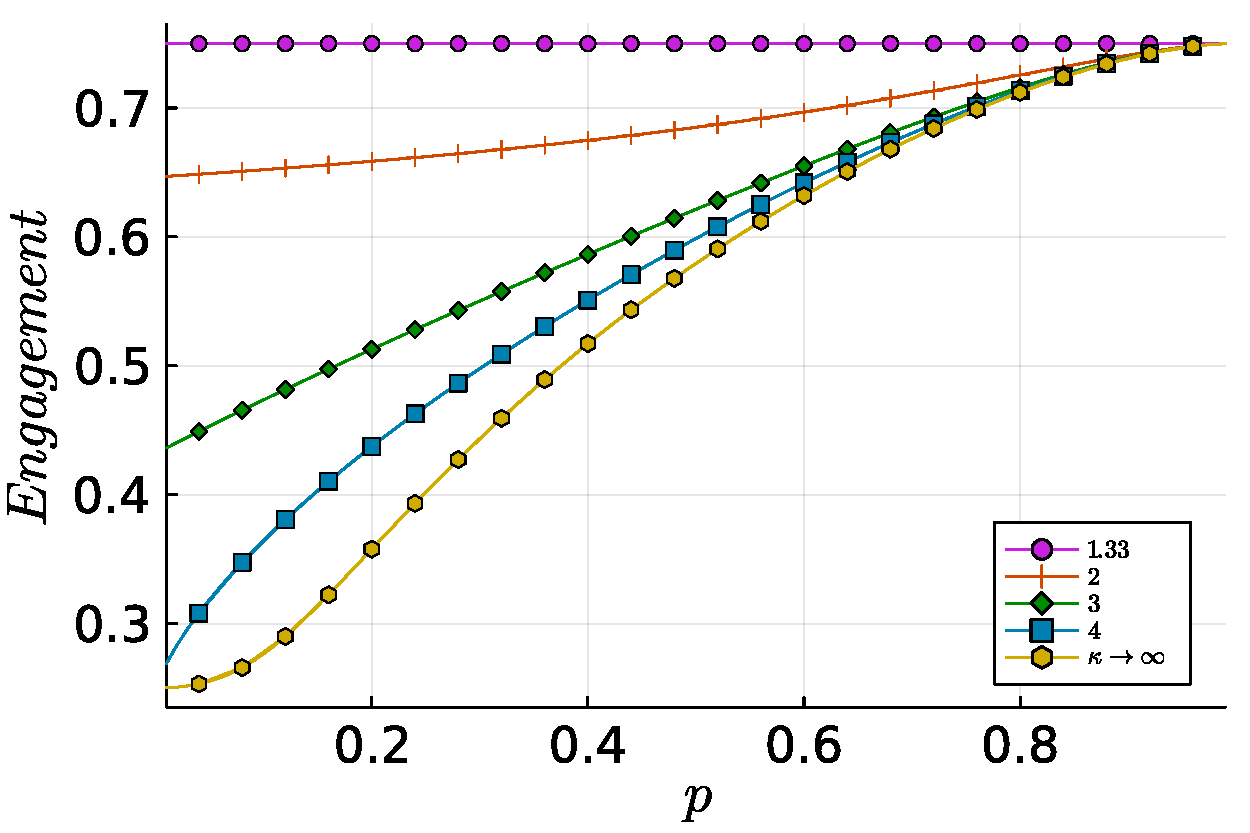
\includegraphics[width=0.22\textwidth]{Figures/engage.pdf}
%     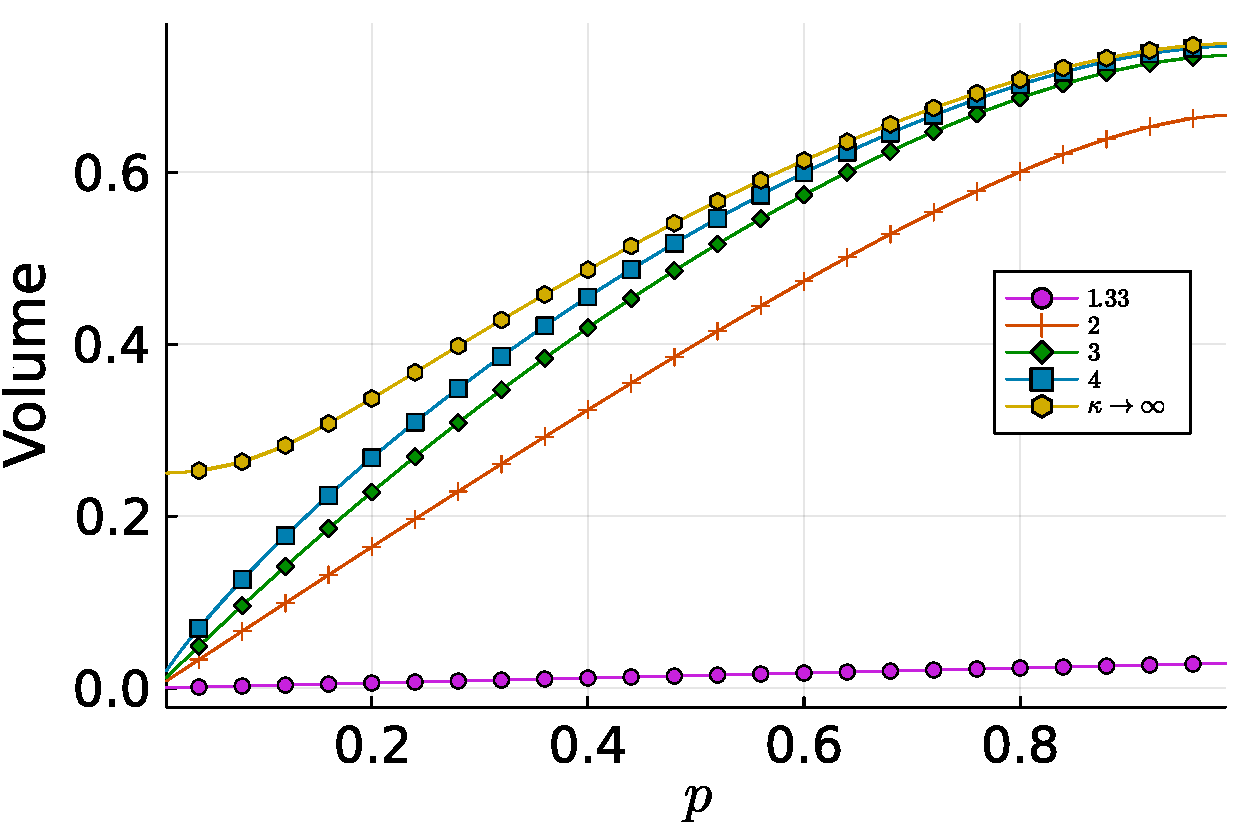
\includegraphics[width=0.22\textwidth]{Figures/volume.pdf}
%     \caption{Caption}
%     \label{fig:misinformation_engagement_volume}
% \end{figure}
\begin{figure}
\centering
\begin{subfigure}{0.3\textwidth}
    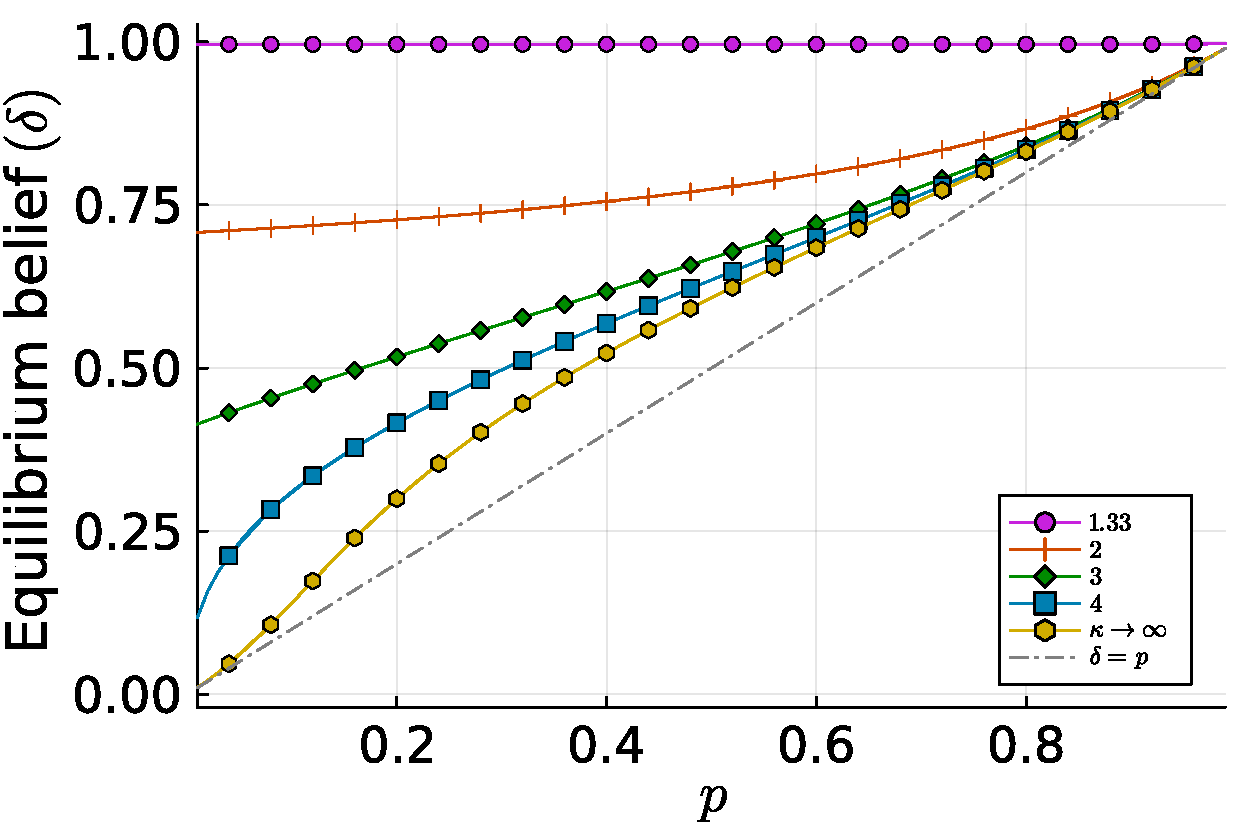
\includegraphics[width = \textwidth]{Figures/p_vs_delta.pdf}
    \caption{}
\end{subfigure}
\vspace{1em}
\begin{subfigure}{0.3\textwidth}
    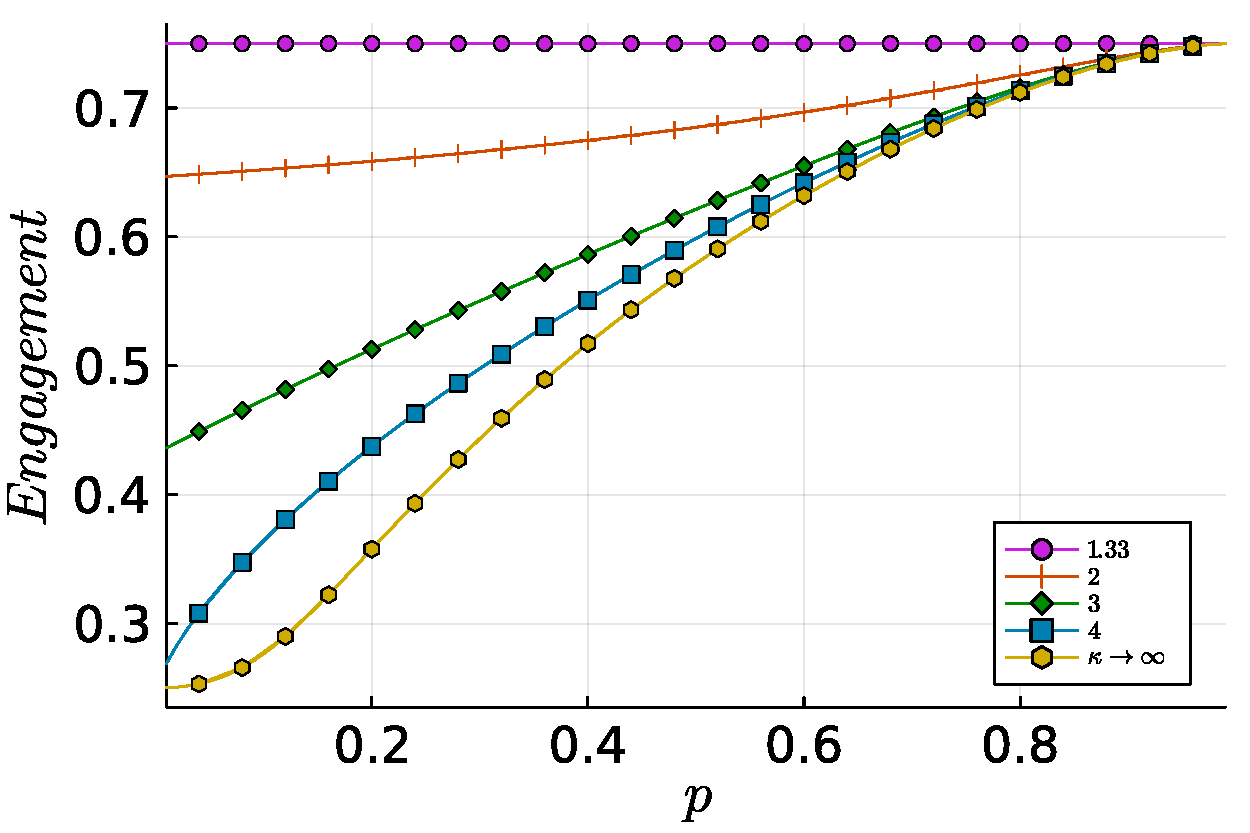
\includegraphics[width = \textwidth]{Figures/engage.pdf}
    \caption{}
\end{subfigure}
\vspace{1em}
\begin{subfigure}{0.3\textwidth}
    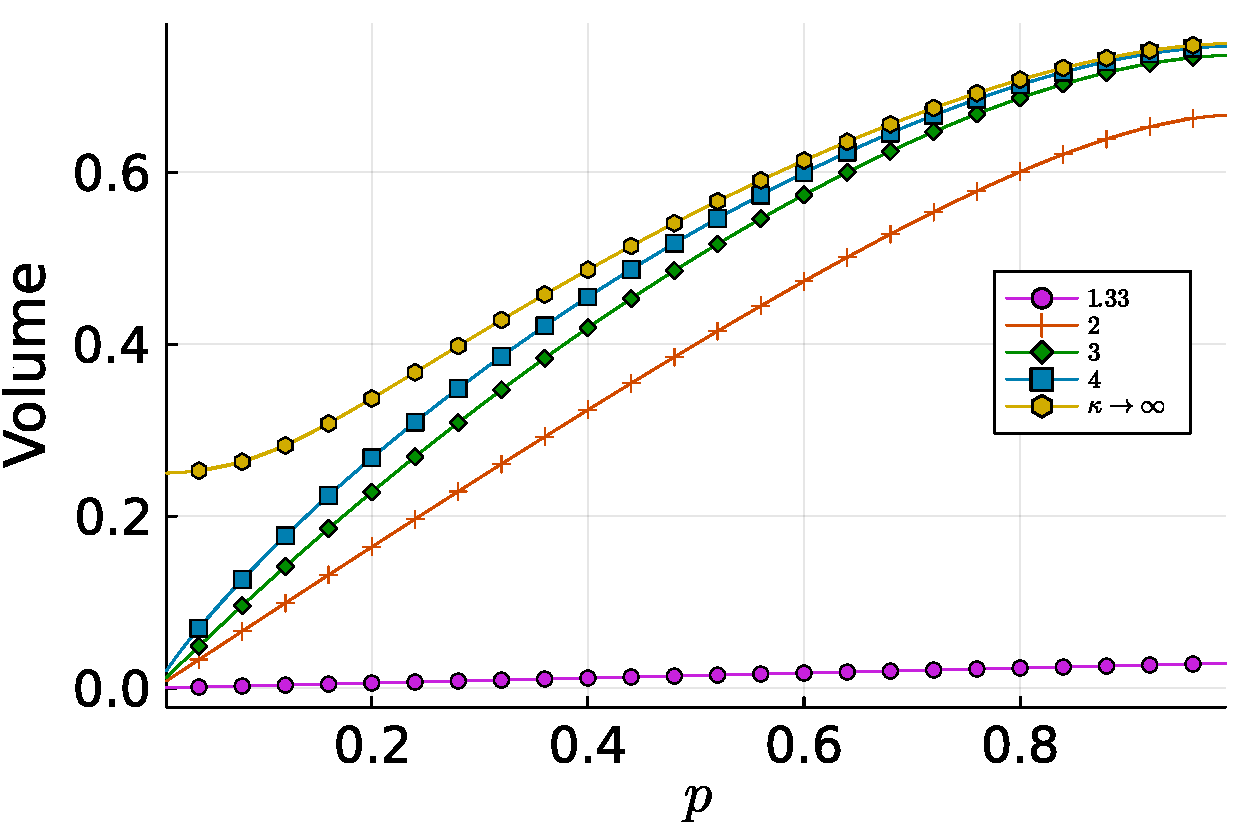
\includegraphics[width = \textwidth]{Figures/volume.pdf}
    \caption{}
\end{subfigure}
    \caption{(a) Average veracity of viral content $\delta$, (b) user engagement level, and (c) volume of viral content in the boom equilibrium as a function of the average veracity $p$ of new content for different values of $\kappa$.}
\end{figure}\label{fig:misinformation_engagement_volume}

Figure~\ref{fig:sensitivity_specificity} (a) shows sensitivity and Figure~\ref{fig:sensitivity_specificity} (b) shows the specificity as a function of the average new content veracity or the fraction of true content entering the system $p$ for different spread factors, $\kappa$. Sensitivity decreases and specificity increases with $p$ because, with increasing $p$, users' beliefs about the veracity of the content increase, and they are more likely to share the content, thus increasing the virality of both true and false content. For $\kappa \geq 2$, the sensitivity/specificity is very high/low for small $p$ because almost all content is never shared and is very low/high for high $p$ because almost all content is always shared. $\kappa = 4/3$ is a critical $\kappa$ given the parameters at which the boom equilibrium emerges. At this value of $\kappa$ the sensitivity is almost $1$ and specificity is $0$ because a negligible fraction of the content goes viral irrespective of the average new content veracity. Sensitivity decreases as $\kappa$ increases, due to higher number of shares leading to higher likelihood virality of all content. However, specificity is non-monotonic in $\kappa$ for low average new content veracity. Increasing $\kappa$ by a small amount above the critical value of $\frac{4}{3}$ gives a big boost to specificity but increasing it further decreases it. This effect is especially important because the sensitivity does not decrease significantly with $\kappa$ for low values of average new content veracity. Thus by appropriately choosing $\kappa$, even for very low values of average new content veracity, peer-filtering effect can be kept very high eliminating a large fraction of false content while allowing a significant fraction of true content to go viral. When the average new content veracity is high then specificity is increasing in $\kappa$. For this analysis, we made a conservative assumption that only a quarter of the population are impartial truthtellers and only half of the population is truthteller. The critical $\kappa$ is lower bounded by $1$ but would increase with the increasing fraction of partisan and impartial truthtellers in the population suggesting that higher values of $\kappa$ can be sustained with high sensitivity and specificity.




\subsubsection{Equilibrium Belief, Engagement, and Volume}
% Figure \ref{fig:misinformation_engagement_volume} (a) shows the average veracity of the content or the fraction of true content present in the system, $\delta$ as a function of the average new content veracity $p$ for different values of $\kappa$. It shows that $\delta$ is at least as big as $p$ suggesting that peer-filtering effectiveness is at least $1$. We note that $\delta$ is very high even for small values of $p$ for small values of $\kappa$. This is because when $p$ is small the users in the social network are more skeptical about the content and only a small fraction of false news goes viral. The difference between $\delta$ and $p$ is the highest when the value of $p$ is moderate or the uncertainty about the content veracity is high. In this range users weigh their private signal about content veracity more introducing the wisdom of the crowds. This demonstrates the power of peer filtering as a solution for fighting misinformation. For higher value of $p$, $\delta$ is naturally high. We also point out that as $\kappa$ increases the peer filtering effect decreases but does not vanish. Peer filtering effect is still present in the limit as $\kappa$ approaches infinity. Figures \ref{fig:misinformation_engagement_volume} (b) and (c) show the user engagement level and the total content volume in the system respectively as a function of the average new content veracity. We find that the user engagement is consistent with $\delta$ suggesting that it may be in platform's interest to keep the misinformation level low on the platform. By appropriately choosing $\kappa$ the platform can both decrease the misinformation level and increase the user engagement without having a significant impact on the volume of content on the platform.
\begin{figure}
    \centering
    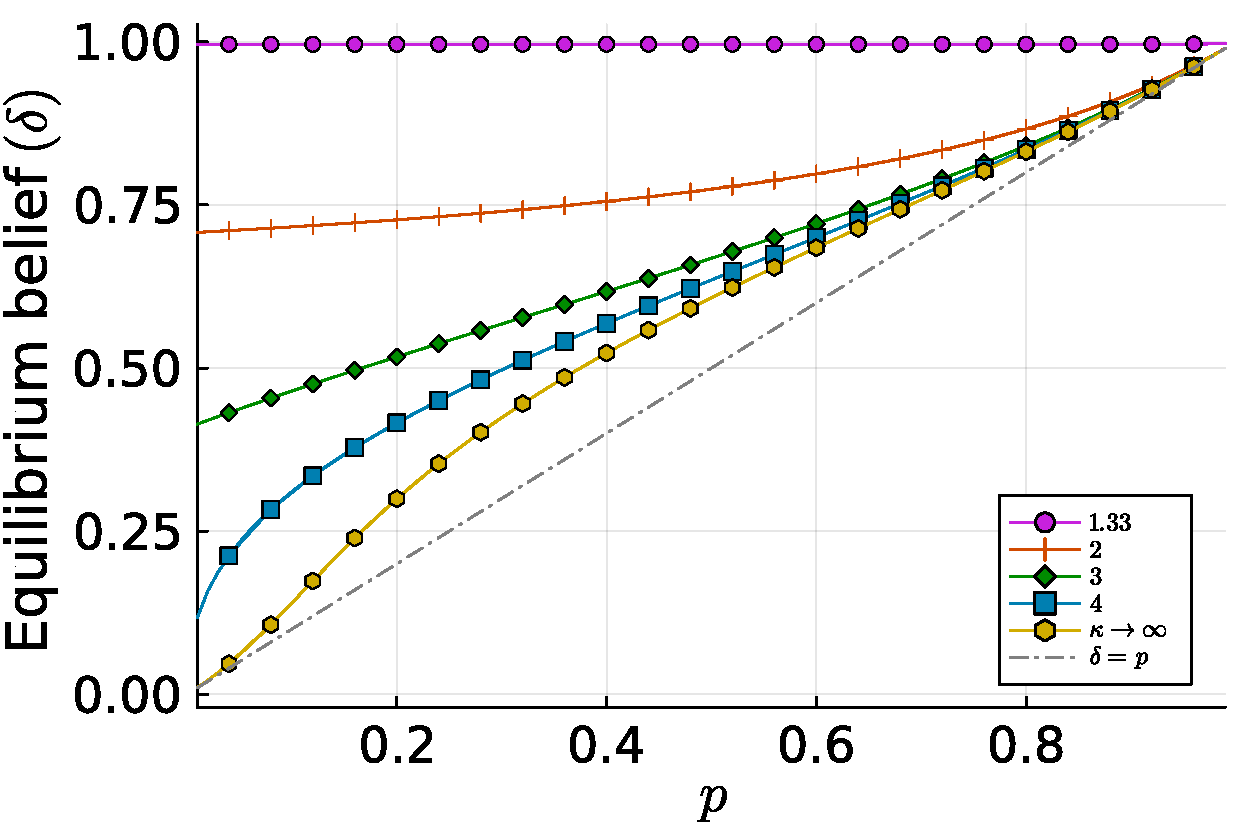
\includegraphics[width=0.3\textwidth]{Figures/p_vs_delta.pdf}
    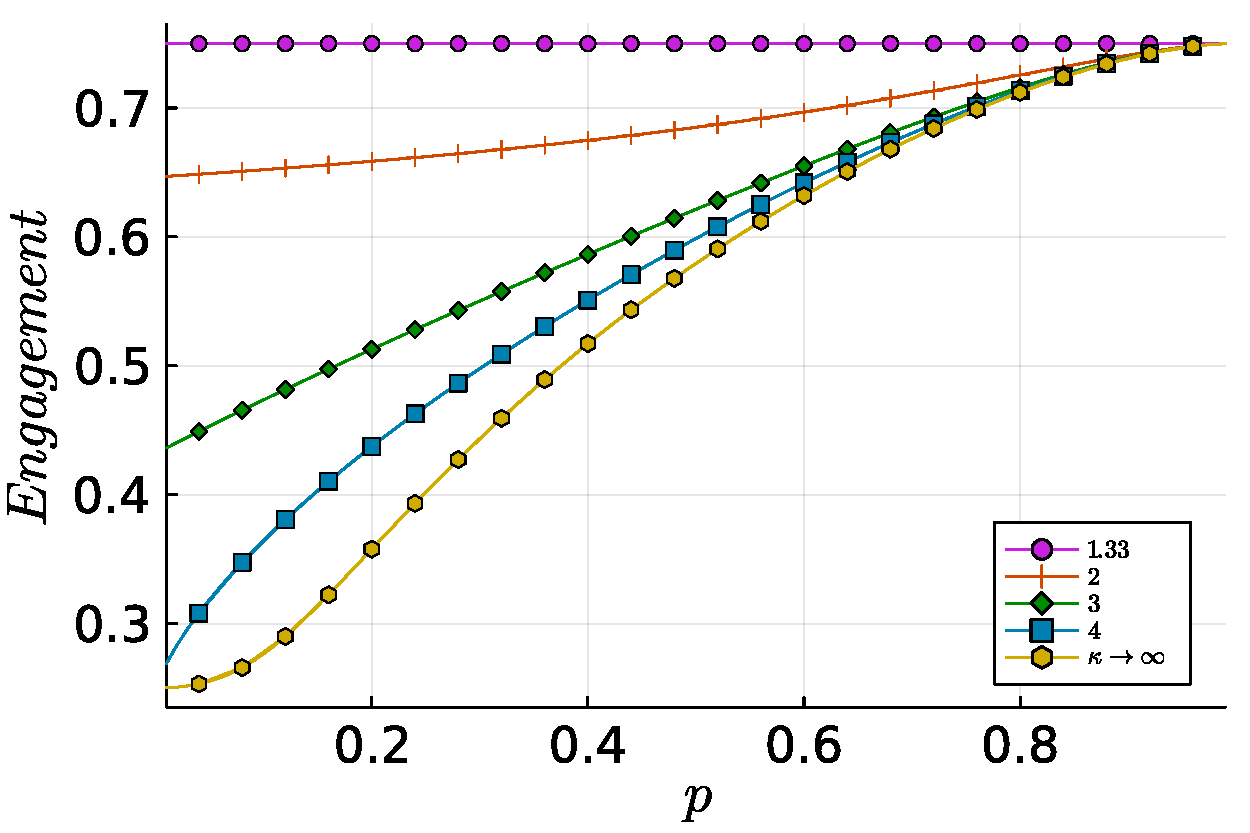
\includegraphics[width=0.3\textwidth]{Figures/engage.pdf}
    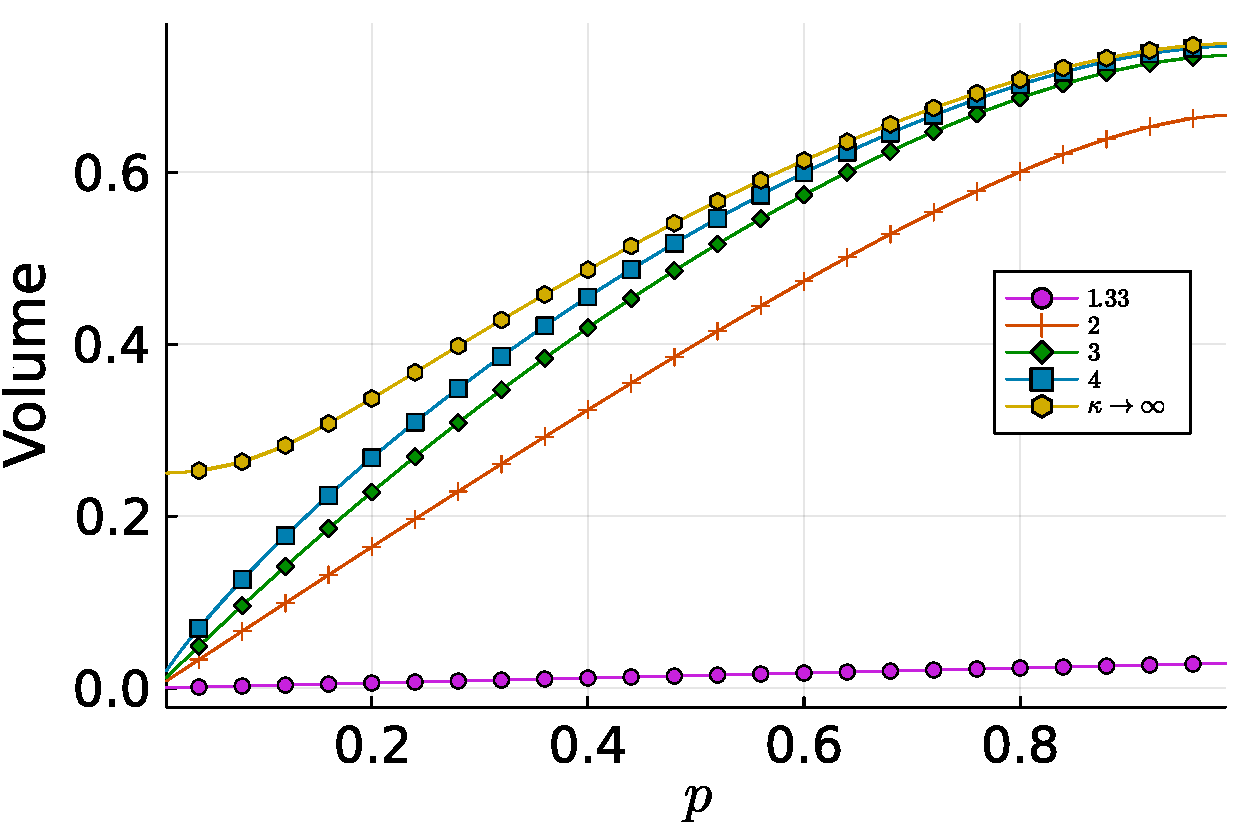
\includegraphics[width=0.3\textwidth]{Figures/volume.pdf}
    \caption{(a) Average veracity of viral content $\delta$, (b) user engagement level, and (c) volume of viral content in the boom equilibrium as a function of the average veracity $p$ of new content for different values of $\kappa$.}\label{fig:misinformation_engagement_volume}
\end{figure}

%% horizontal does cost space
% \begin{figure}
%     \centering
%     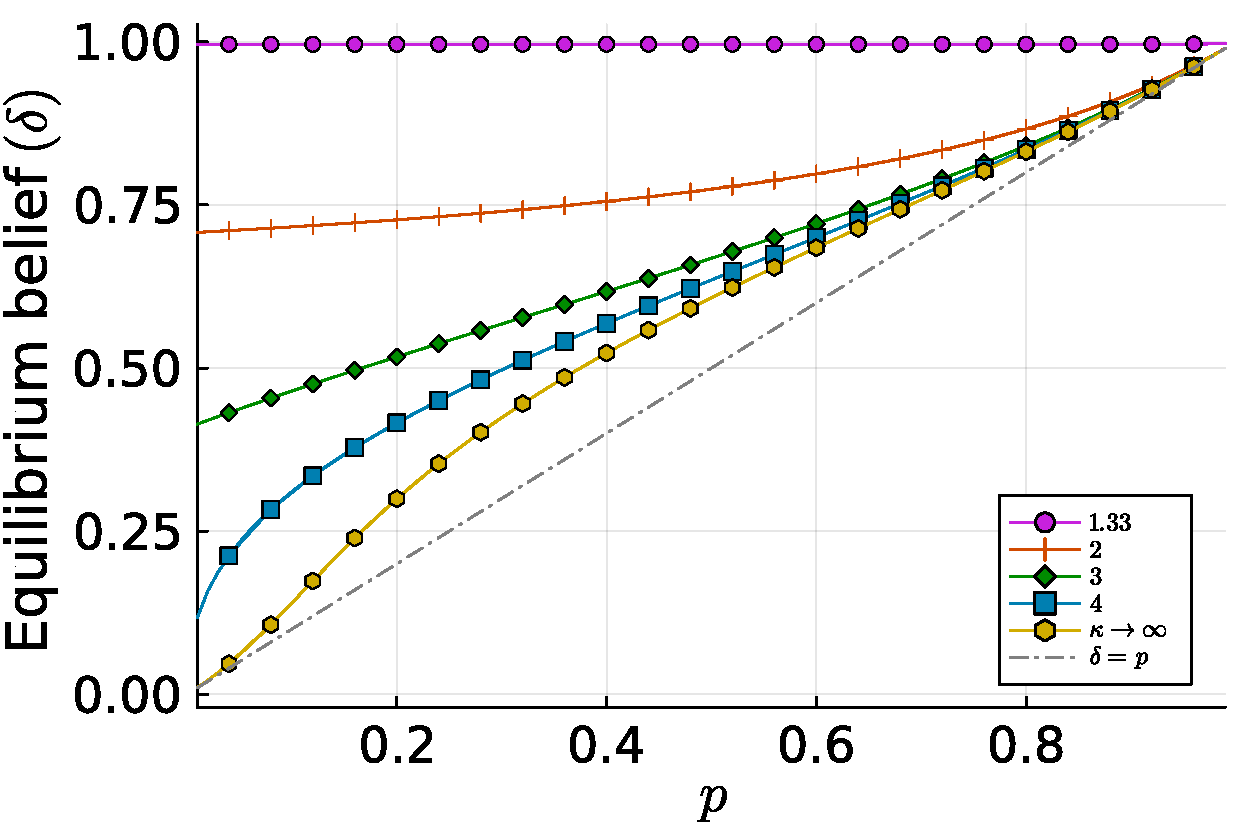
\includegraphics[width=0.22\textwidth]{Figures/p_vs_delta.pdf}
%     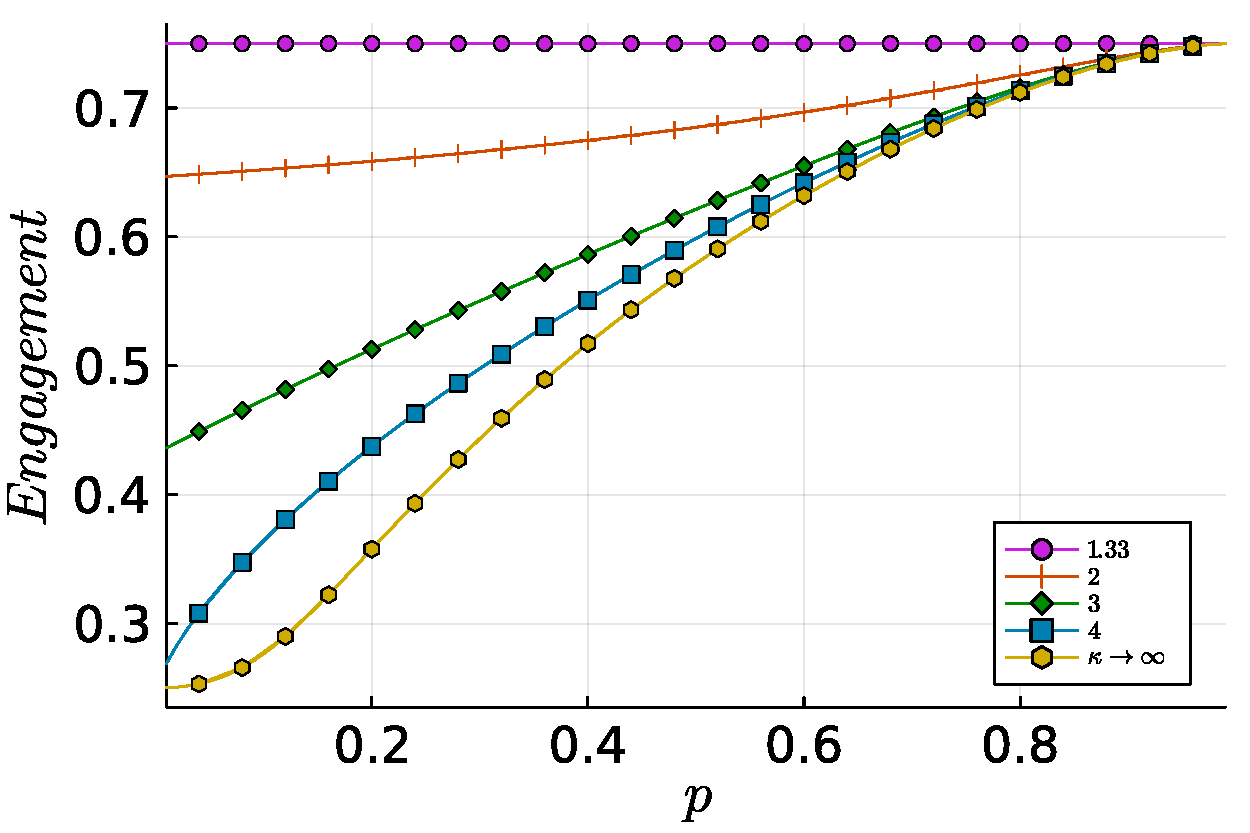
\includegraphics[width=0.22\textwidth]{Figures/engage.pdf}
%     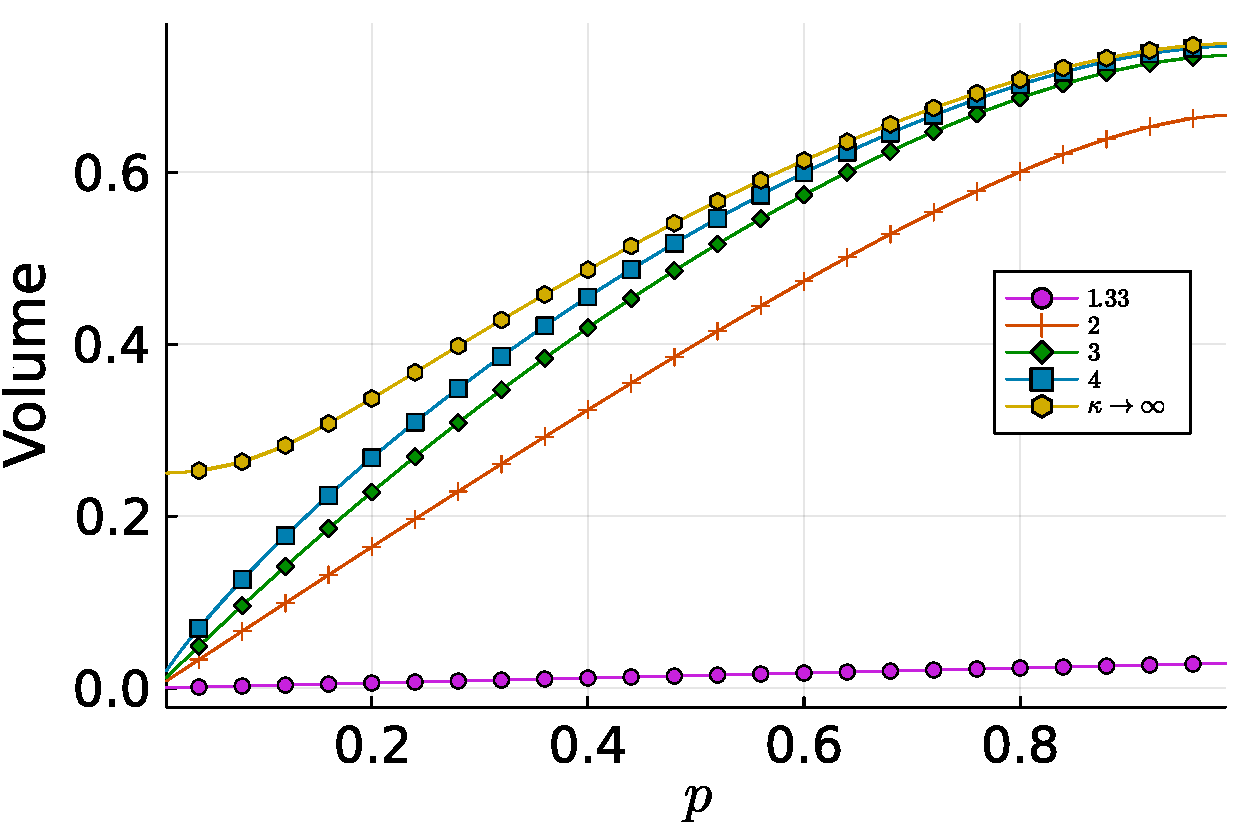
\includegraphics[width=0.22\textwidth]{Figures/volume.pdf}
%     \caption\left(a) Average veracity of viral content $\delta$, (b) user engagement level, and (c) volume of viral content in the boom equilibrium as a function of the average veracity $p$ of new content for different values of $\kappa$.}
%     \label{fig:misinformation_engagement_volume}
% \end{figure}

Additional numerical results on peer filtering effect with general type distributions are provided in Appendix~\ref{sec:gentyperes}.


\section{Generalizations}\label{sec:generalizationPaper}
% Our main model makes various modeling choices (the specific signal structure, the deterministic peer sharing model, and no homophily) for simpler exposition and for establishing equilibrium existence. In the appendix, we show how this model can be generalized in several ways. In Subsection~\ref{sub:signal_structure}, we establish that our structural results on the equilibrium hold under very general signal structures. Similarly, in Subsection \ref{sub:randomBoom}, we generalize our results to the setting where $\kappa$ is random. Finally, in Subsection~\ref{sec:homophil}, we extend our network model to incorporate homophily and study its impact on the peer filtering effect. 
% % \erdelete{Some portions of the model were instantiated with particular choices for purposes of  exposition as well as to provide detailed theorems. In the Appendix \ref{sec:generalization}, we show how two of these choices can be generalized and still leave insights of this work intact. We study three generalizations. The first generalization is regarding the choice of signal distribution as in Equation $\ref{eq:signal-dist}$. We show what conditions are needed on the signal structure for true content to spread further than false content. The second generalization is to allow the number of shares, $\kappa$ to be random. This is important because the thresholds for different equilibrium structure in Theorem \ref{thm:equilibria-existence} are not necessarily integer. With a random number of shares, the thresholds may depend upon a statistic instead of $\kappa$ itself. In particular interest is the condition for existence of boo equilibrium. We show that when $\kappa$ is random then conditions  for the boom-equilibrium in Theorem \ref{thm:equilibria-existence}, are satisfied when $\kappa$ is replaced by $\ex{[\kappa]}$. The third generalization introduces homophily in network structure. Social networks demonstrate some level of homophily, so it is important to study the impact of homophily and local diffusion heterogeneity on the strength of peer-filtering effect. We generalized our homogeneous random network model to a model with left and right communities with a variable level of mixing between the communities. Through this variable we control the level of homophily in the network. We find the increasing homophily reduces the average veracity of the content in the network but the peer filtering effect is still strong. The impact of homophily is high when $\ex{[\kappa]}$ is low and weakens as $\ex{[\kappa]}$ increases. In the limit, the impact of homophily vanishes. In all cases the average veracity of the content in the network is higher than the content introduced to the network due to the peer filtering effect.}

\subsection{Generalized signal structure}\label{sub:signal_structure}
%% This is directly a copy of what Dr. Iyer wrote
In this subsection, we explore how dependent the primary results are to the assumption of a specific ``signal structure''. By signal structure, what we mean is a set of signals that the users can receive and the distributions in which these signals arise for true and false content. Below is a formal definition. 
\begin{definition}
    A signal structure is a tuple $(S, \Sign,  \prob_\true, \prob_\false)$, where $(S, \Sign)$ is a standard Borel space and $\prob_\true$ and $\prob_\false$ are measures on $(S, \Sign)$.
\end{definition}
The interpretation of a signal structure $\Sigma = (S, \Sign, \prob_\true, \prob_\false)$ is as follows: the set $S$ represents the set of values taken by a user's private signal  obtained from consuming a content. This signal is assumed to be distributed according to the distribution $\prob_\true$ if the content is true, and according to the distribution $\prob_\false$ if the content is false. Specifically, letting $(\tilde{\alpha}, \tilde{s})$ denote respectively a content's veracity and the signal received by an user upon consuming a content, we have $\prob(\tilde{s} \in B | \tilde{\alpha} = \true) = \prob_\true(B)$ and $\prob(\tilde{s} \in B | \tilde{\alpha} = \false) = \prob_\false(B)$ for all $B \in \Sign$.

Given a signal structure $\Sigma = (S, \Sign, \prob_\true, \prob_\false)$ and $\mu \in [0,1]$, we let $\prob_{\mu}^{\Sigma}$ denote the measure where, if $(\tilde{\alpha}, \tilde{s}) \sim \prob_{\mu}^\Sigma$, then with probability $\mu$, we have $\tilde{\alpha} = \true$ and $\tilde{s} \sim \prob_\true$ and with probability $1 - \mu$, we have $\tilde{\alpha} = \false$ and $\tilde{s} \sim  \prob_{\false}$. When the signal structure $\Sigma$ is clear from context, we drop the superscript on $\prob_\mu^\Sigma$. Finally, we have the following definition:
\begin{definition} Given a signal structure $\Sigma = (S, \Sign, \prob_\true, \prob_\false)$, a standard Borel space $(S', \Sign')$ and a measurable mapping $f : S \to S'$, we define the pushforward signal structure $\Sigma_f$ as the signal structure $(S', \Sign', \prob_\true', \prob_\false')$, where $\prob_\true'$ and $\prob_\false'$ are the pushforwards by $f$ of   $\prob_\true$ and $\prob_\false$ respectively, i.e., for any $B \in \Sign'$, $\prob_\alpha'( B) = \prob_\alpha\left( f^{-1}(B)\right)$ for each $\alpha \in \{\true, \false\}$. (Note that if $(\tilde{\alpha}, \tilde{s}) \sim \prob_{\mu}^\Sigma$ and $\tilde{u} = f(\tilde{s})$, then $(\tilde{\alpha}, \tilde{u}) \sim \prob_\mu^{\Sigma_f}$.)  
\end{definition}

With this definition in place, the following lemma shows that from any signal structure, one can construct an {\em equivalent} signal structure satisfying certain fundamental properties. 
\begin{lemma}\label{lem:sign_equiv}
  For any signal structure $\Sigma = (S, \Sign, \prob_\true, \prob_\false)$  there exists a Borel measurable mapping $f : S \to [0,1]$ such that the pushforward signal structure  $\Sigma_f = ([0,1], \mathcal{B}[0,1], \hat{\prob}_\true, \hat{\prob}_\false)$ satisfies the following properties. 
  \begin{enumerate}
    \item For all $\mu \in [0,1]$, we have (a.s.) $\prob_\mu(\tilde{\alpha} = \true | \tilde{s} = s) = \prob_\mu ( \tilde{\alpha} = \true | \tilde{u} = f(s))$.
      \item For almost all $u \in [0,1]$, we have $\prob_{\sfrac{1}{2}} (\tilde{\alpha} = \true |\tilde{u}=u)=u$, and
      \item $\hat{\prob}_\true$ first-order-stochastically-dominates $\hat{\prob}_\false$.
  \end{enumerate}
\end{lemma}
The preceding result states that for any signal structure, there exists an equivalent signal structure with signals in the interval $[0,1]$. In particular, part (1) of the lemma statement states that, regardless of a user's prior belief about content veracity, her posterior belief upon receiving a signal $\tilde{s} = s$ under the signal structure $\Sigma$ is the same as her posterior belief upon receiving the signal $\tilde{u} = f(s)$ under the pushforward signal structure $\Sigma_f$. Thus, it is without loss of generality to focus on the structure $\Sigma_f$. For such a signal structure, if a content is {\em a priori} equally likely to be true or false, then the signal represents the posterior belief that the content is true (as stated in part (2)).  Finally, under the signal structure $\Sigma_f$, we have the property that higher signals are more likely when the content is true than when the content is false (as follows from part (3)). 

The set of properties listed in parts (2) and (3) of the lemma statement are sufficient for establishing many of the structural results on the equilibrium in our model. We state this result more precisely in the following proposition.
\begin{proposition}
For any signal structure satisfying properties (2) and (3) in Lemma~\ref{lem:sign_equiv}, all the results in Section~\ref{sec:user_behavior} (namely, Theorem~\ref{thm:threshold} and Proposition~\ref{prop:beta-monotonicity}) and all results in Section~\ref{sec:spread-equilibrium} on equilibrium structure (namely, Theorems~\ref{thm:boom-bust},~\ref{thm:delta_geq_p}~and~\ref{thm:kappa-thresholds}) continue to hold. 
\end{proposition}
The preceding proposition can be established by noticing that the proofs of the listed results only use the stated properties, and do not use the explicit structure of the signal distribution. On the other hand, it is in Theorem~\ref{thm:equilibria-existence} that we use the explicit structure of the signal distribution for establishing equilibrium existence, and for computing the specific thresholds on $\kappa$ under which the different equilibrium regimes emerge. These latter results are important for our numerical analysis in Section~\ref{sec:Peer_filtering}. While similar equilibrium regimes may persist under more general signal distributions, more structure on the signal distribution is needed to establish it as well as to characterize the structure of these regimes.

\subsection{Boom-Equilbria under Random \texorpdfstring{$\kappa$}{k}}\label{sub:randomBoom}
In this subsection, we examine the setting where a random number of peers observe the content when a user shares it.  Here, the number of shares, $\kappa$, is a discrete random variable with bounded support.  When a user decides to share a piece of content it is shown to $k$ users with probability $\pi_k$. We denote the maximum number of users it could be shown to as $\kappa_{\max}$.   In this case, the probability that a content with veracity $\alpha$, introduced at a random user in the network, will go bust, $1 - q^{\alpha}$, is given by the following fixed point equation.
\begin{equation}\label{eq:non-det-viral-prob}
    1 -q^\alpha = 1 - \beta^\alpha + \beta^\alpha\sum_{k=1}^{\kappa_{\max}} \pi_k {\left(1 - q^\alpha\right)}^k 
\end{equation}

This equation differs from equation~\eqref{eq:viral-prob} for the deterministic $\kappa$ in the second term on the right hand side. In particular, ${\left(1-q^\alpha\right)}^\kappa$ for the deterministic case was replaced by $ \sum_{k=1}^{\kappa_{\max}} \pi_k {\left(1 - q^\alpha\right)}^k $ for the random case. Each term of this summation is the joint probability, given a user shares the content, that the content is shared with $k$ peers and the network spread process starting from each of the $k$ peers go bust. 

We can now characterize the conditions for the boom equilibrium when $\kappa$ is random. Since, the comparative statics of the peer filtering phenomenon is mostly governed by the boom equilibrium properties, we focus only on the boom equilibrium. We find a sharp condition for the existence of the boom equilibrium as stated in the following theorem.

\begin{theorem}\label{thm:non-det-kappa}
    When $\kappa $ is a discrete random variable then there exists a boom equilibrium if and only if  $\ex{\kappa} > \frac{2 }{1 + \tm}$
\end{theorem}

We note that the condition for the existence of the boom equilibrium is similar to the condition when $\kappa$ was deterministic, although the threshold for the existence now applies to the expected value of $\kappa$. The threshold $\frac{2}{1+ \tm}$ in the preceding theorem is same as in Theorem~\ref{thm:equilibria-existence}. This implies that certainty equivalence for the threshold holds for the existence condition. We note that the exact equilibrium will depend upon the full distribution of $\kappa$ and higher order statistics, beyond the expectation, will impact the virality of true and false content $q^\true, q^\false$ in equilibrium. In order to show that no boom equilibrium will exist when $\ex{\kappa} \leq \frac{2}{1+\tm}$, we show that the branching factor of the spread process is less than one and the size of the spread is finite, suggesting that the content will almost surely go bust in large networks. The proof of the existence of the boom equilibrium when $\ex{\kappa} > \frac{2}{1+\tm}$ follows similar logic as the proof of Theorem~\ref{thm:equilibria-existence} but needs a little more care due to randomness of $\kappa$. Here again, we consider two cases, when $\ex{\kappa} \geq \frac{2}{1-\tt}$ and $\ex{\kappa} \in (\frac{2}{1+\tm}, \frac{2}{1-\tt})$. For both cases, we establish the the continuity of $\Pi(\delta)$ and that there are some values of $\delta \in (0, 1) $ where $\Pi(\delta) < \delta$ and for other values of $\delta \in (0, 1) $ where $\Pi(\delta) > \delta$. The fixed point condition is then satisfied by the intermediate value theorem as in the proof of Theorem~\ref{thm:equilibria-existence}.

\subsection{Homophily}\label{sec:homophil}
In this section, we will discuss an extension where homophily is added. Following this model reformulation, we perform a brief numerical study.  Homophily here will refer to a natural clustering the connections of left-leaning users with other left-leaning users and right-leaning users with right-leaning users. We model this as number of one's peers that share the same inclination, $\lambda$, as distributed by $Bin(\kappa, f_{in})$ where $f_{in}$ is probability that any particular connection is from the same inclination. We will call $f_{in}$ the mixing level. If the mixing level is exactly $\frac{1}{2}$ then we obtain the previous case, shared content is equally likely to be seen by left and right-learning users. This fact will be carefully shown later.  On the other hand, when $f_{in} > \frac{1}{2}$, is the case with homophily, as users are more likely to have connections to other like-minded users. Although the compositions of one's peers have changed, we will still assume that a piece of content external to the system is shown to any user uniformly at random. 

What directly changes in this model is that when a user chooses to share, a biased fraction of the receiving users will have the same inclination as the sharer. In order to track this, we will work with the probability that user shares content that given that it is aligned or misaligned with them.  These probabilities are denoted by
\begin{align}\label{eqn:new_share_prob}
\beta^\alpha_{\alg} &= \sum_{t \in \Theta} \theta_t \beta_{\alg, t}^\alpha  \\
\beta^\alpha_{\mal} &= \sum_{t \in \Theta} \theta_t  \beta_{\mal, t}^\alpha 
\end{align}

The probability that content goes viral is similar to before, but depends on what ``state'' it is in. The two states are either it is currently being viewed by an aligned user or a misaligned user. Let $q^\alpha_\alg$ refer to the probability that content that starts with an aligned user goes viral and $q^\alpha_\mal$ refer to the probability that content starting with a misaligned user goes viral. We get two systems of equations given by:
\begin{align}\label{eqn:new-fixed}
    1-q_\alg^\alpha = 1 -\beta^\alpha_\alg + \beta^\alpha_\alg \ex{\left(1-q_\alg^\alpha\right)^{\lambda} \left(1-q^\alpha_\mal\right)^{\kappa - \lambda}} \\ 
     1-q_\mal^\alpha = 1 -\beta^\alpha_\mal + \beta^\alpha_\mal \ex{\left(1-q_\mal^\alpha\right)^{\lambda} \left(1-q^\alpha_\alg\right)^{\kappa - \lambda} }
\end{align}

This can be interpreted as accounting for how content fails to go viral in two ways. The left side is the expression for not going viral. The right side is the chance that content is not shared the first time plus the probability it is shared but does not go viral. To not go viral after being shared it must be that each of the spreads starting at each of the $\lambda$ same group users and the $\kappa - \lambda$ different group users fail to go viral. 

Next, we can express the new proportion of true content a user sees as
\begin{equation*}\label{eq:homophil_eqi}
    \Phi = \frac{p ( q_\alg^\true + q_\mal^\true) }{p ( q_\alg^\true + q_\mal^\true) + (1-p) ( q_\alg^\false + q_\mal^\false)}
\end{equation*}

Finally, we can redefine what it means to be an equilibrium in the case of homophily. It is similar to before, but now reflects the change in sharing probabilities and of going viral. 

\begin{definition} An equilibrium is given by sharing probabilities $(\beta^\alpha_\alg, \beta_\mal^\alpha : \alpha \in \{\true, \false\})$ and a prior belief $\delta  \in (0,1)$, such that  (i) given the prior belief $\delta$, the sharing probabilities $\beta^\alpha_\alg, \beta^\alpha_\mal$ are obtained from~\eqref{eqn:new_share_prob}; and (ii) given the sharing probabilities $\beta_\alg^\alpha, \beta_\mal^\alpha$, the prior belief $\delta$ satisfies $\delta = \Phi(\beta^\true, \beta^\false)$, where $\Phi(\beta_\alg^\true, \beta_\mal^\true, \beta_\mal^\false, \beta_\mal^\false)$ is given by~\eqref{eq:homophil_eqi}. Taken together, in an equilibrium, the prior belief $\delta$ satisfies the fixed-point equation $\delta = \Phi\left(\beta_\alg^\true(\delta), \beta_\mal^\true(\delta), \beta_\mal^\false(\delta), \beta_\mal^\false(\delta)\right)$.
\end{definition}

The key metrics also change slightly. Now the volume level, the amount of total viral content, is $\frac{1}{2} \left( p (q_\alg^\true + q_\mal^\true) + (1-p)(q_\alg^\false + q_\mal^\false) \right) $. The $\frac{1}{2}$ is coming from the $\frac{1}{2}$ chance that arriving content is aligned or misaligned. Likewise, the engagement level is now $\frac{1}{2} \left( \delta (\beta^\true_\alg + \beta^\true_\mal) + (1-\delta) (\beta^\false_\alg + \beta^\false_\mal) \right)$. 

\subsubsection{Relationship between models}

Previously, we claimed that the setting $f_{in} = \frac{1}{2}$ reduces to the standard model. However, it is not obviously true. One reason of concern is that in the fixed point equation for $q^\alpha$ is split into ${\left(1-q^\alpha\right)}^\kappa $ into $\ex{ \left(1-q_\alg^\alpha\right)^\lambda {\left(1-q_\mal^\alpha\right)}^{\kappa -\lambda} } $. The natural requirement is that in this setting the average of $q_\alg^\alpha, q_\mal^\alpha$ is $q^\alpha$. What we will show is that this is in case.  
\begin{proposition}
    Let $f_{in} = \frac{1}{2}$ and fix $\delta$. Then if $q^\alpha$ is the solution to Equation~\ref{eq:viral-prob} and $q_\alg^\alpha$ and $q_\mal^\alpha$ the solutions to Equations~\ref{eqn:new-fixed} then 
    \[q^\alpha = \frac{1}{2} \left(q_\alg^\alpha + q_\mal^\alpha \right)\]
\end{proposition}
\begin{proof}
    Let $(I, T)$ denote a user's type, where $I \in \{\alg, \mal\}$ denotes the users inclination (with respect to a fixed content), and $T \in \{IT, PT, PF, IF\}$. Assume $\kappa$ is a deterministic integer. Let $(I_i, T_i)$ denote the $ith$ peer's type. 

    The most refined analysis, keeping track of the full user type

    \[ 1 - q_{(I,T)}^\alpha = 1 - \beta_{(I,T)}^\alpha + \beta_{(I,T)}^\alpha \ex{  \prod_{i=1}^\kappa  (1 - q_{(I_i, T_i)}^\alpha )  |  (I,T) }. \] 

   Now, in general $(I_i, T_i)$ are all iid conditional on $(I, T)$. So, we can interchange the expectation and the product to get 

    \[ 1 - q_{(I,T)}^\alpha = 1 - \beta_{(I,T)}^\alpha + \beta_{(I,T)}^\alpha    \left(1 - \ex{ q_{(I_i, T_i)}^\alpha   | (I, T)  } \right)^\kappa. \] 

    When $f_{in} = \frac{1}{2}$, $(I_i, T_i)$ are unconditionally independent (and independent of $(I,T)$). So, we get

     \[ 1 - q_{(I,T)}^\alpha  = 1 - \beta_{(I,T)}^\alpha  + \beta_{(I,T)}^\alpha  \left(1 - \ex{ q_{(I_i, T_i)}^\alpha}\alpha\right)^\kappa. \]

    Taking expectation over $(I, T)$ gives us our original equation with $q^\alpha = \ex{ q_{(I, T)}^\alpha}$ and $\beta = \ex{ \beta_{(I, T)}}$. 

    When $f_{in} \neq 1/2$, then $I$ and $I_i$ are not independent, but $T_i$ and $(I, T)$ are still independent. In particular, after taking expectation over $T$ we get the set of equations:
    \begin{align*}
    1 - q_A &= 1 - \beta_A + \beta_A \left(1 - f_{in} q_A - f_{out} q_M\right)^\kappa 
    1 - q_M &= 1 - \beta_M + \beta_M \left(1 - f_{in} q_M - f_{out} q_A\right)^\kappa 
    \end{align*}
where $q_I = \ex{ q_{(I, T)}| I }$ and $\beta_I = \ex{ \beta_{(I,T)} | I}$. 
\end{proof}

\subsubsection{Numerical Simulation}

Here, we perform a numerical study of the resulting equilibrium belief in the case of homophily. Throughout this section, we set $p$, the average veracity of the incoming content, to $\frac{1}{2}$ and the types to be evenly distributed, so that $\theta_{IT} = \theta_{PT} =\theta_{IF} = \theta_{PF} = \frac{1}{4}$. For a variety of $\kappa$s we will vary $f_{in}$ to make the network more or less homogeneous. 

\begin{figure}[h]
    \centering
    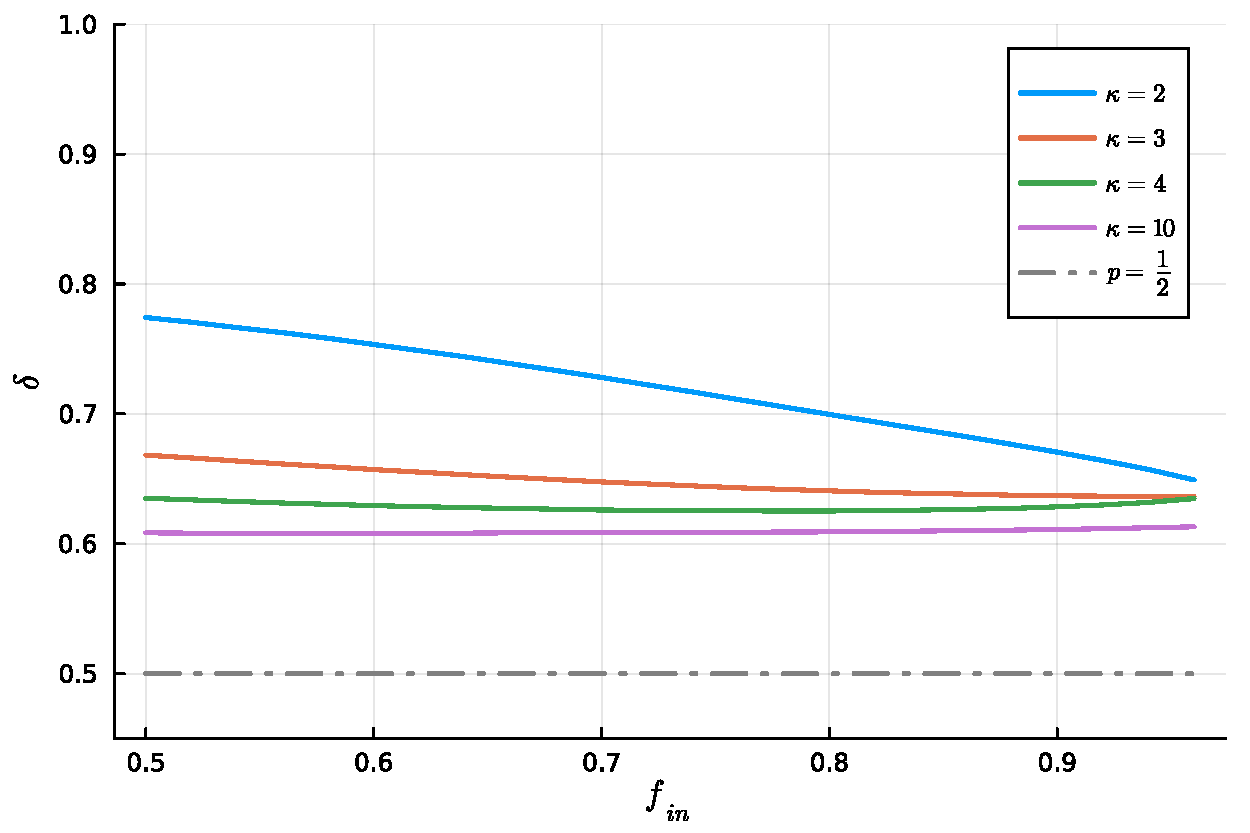
\includegraphics[width=0.5\linewidth]{Figures/vsfin.pdf}
    \caption{Equilibrium belief as a function of homophily for a variety of $\kappa$}\label{fig:vsfin}
\end{figure}

In Figure~\ref{fig:vsfin}, we plot the equilibrium belief as a function of how much homogeneity there is in the network. As $f_{in}$ increases, the equilibrium belief for low $\kappa$ decreases. The reason for this is the peer filtering effect. As it becomes easier for false content to go viral, users self-moderate and become more skeptic by adjusting their prior belief downwards. But curiously, as $\kappa$ increases, we find that $\delta$ can increases in $f_{in}$. Furthermore, we find that larger $\kappa$ induces a more stable response to changes in $f_{in}$. The reason to expect this flattening is that when $\kappa$ is very large, the probability of sharing is governed largely by the probability of the first user sharing. If they do then the content will be shown to enough users that it is likely to go viral which makes who they share to less important. 


\begin{figure}
    \centering
    \begin{subfigure}{0.45\textwidth}
        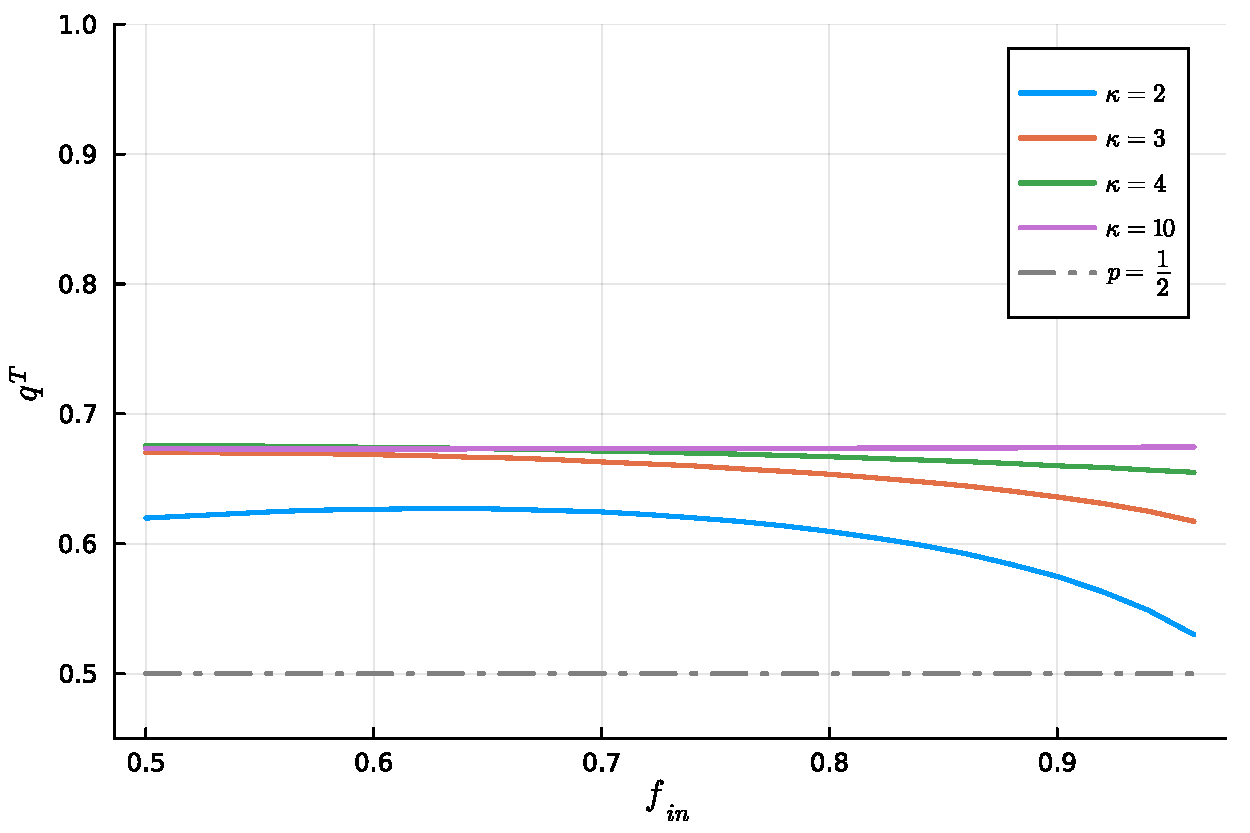
\includegraphics[width=\textwidth]{Figures/qtvsfin.pdf}
    \end{subfigure}
    \begin{subfigure}{0.45\textwidth}
        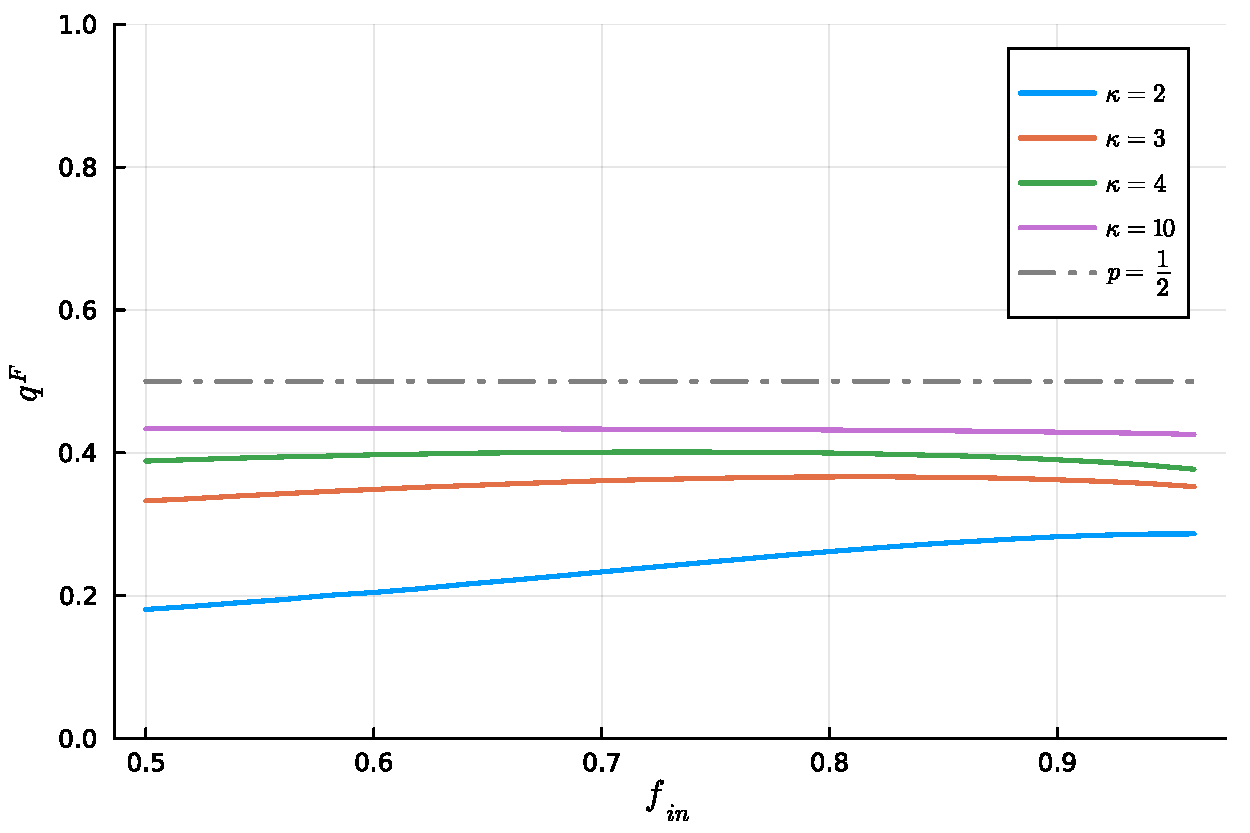
\includegraphics[width=\textwidth]{Figures/qfvsfin.pdf}
    \end{subfigure}
    \caption{$q^\true$ and $q^\false$ }\label{fig:new_qs}
\end{figure}
The reason for this difference is better explained by looking at how $\frac{1}{2} \left( q^\true_\alg + q^\true_\mal\right)$ and $\frac{1}{2} \left( q^\true_\alg + q^\true_\mal\right)$ each change. These should be regarded as the average virality of true and false content respectively. In Figure~\ref{fig:new_qs}, plot these metrics. We first observe that for larger $\kappa$, both metrics are more stable under homophily changes. Looking specifically at the most volatile case, $\kappa=2$, we see that false content is becoming more viral with an increasingly polarized community structure. But when we look at true content we see the opposite, virality is decreasing with polarization. There are two competing effects in play. A high polarization leads to misaligned content (with respect to the first sharer) being surprised, and aligned content to be promoted. But they do not have to affect the virality evenly. Here we see that when the sharing probability is already low, the case for false content,  more total content can go viral. But, when the sharing rate is higher, the case for true content, the net effect is a decreased virality due to true, misaligned content being suppressed outweighing the effect of true and aligned content being promoted. 
% s that users treat true and false content in a more similar way.  





% We observe that as $\kappa$ increases, the equilibrium belief decreases. This like the standard case is because it is is easier for all content to go viral as $\kappa$ increases, but false content gains comparatively more virality from an increase in $\kappa$. What we also observe is that at all levels of $f_{in}$, with larger $\kappa$, the equilibrium beliefs converge to the same value. 



% Next, we show how a different mixing level changes the response seen in to a change in $\kappa$. When considering possible network interventions, this is a more natural question, since $\kappa$ can be modified by the platform but the composition of ones peers is harder for the platform to change. 

% FIGURE HERE 


% What we observe is that as the network gets more homophily, the equilibrium belief decreases. This is in line with what the previous sections suggest. As homophily increases, it becomes more likely that users are willing to share content with a low signal because it aligns with them and all users regardless of types would weakly prefer to share aligned content over misaligned content with the same signal. Below, we plot the usage metrics for this experiment. 

% FIGURE HERE

% As suggested, we see that the volume of viral content is increasing in the amount of homophily. 

\section{Peer Filtering under General Type Distributions}\label{sec:gentyperes}
Here we study how the type distribution $\theta$ affects the key performance metrics. Throughout this section we will fix $\kappa=3$. This choice is sufficiently large so as to guarantee a boom equilibrium always exists throughout the entire parameter space. This is a result of Theorem~\ref{thm:equilibria-existence} which says that a boom equilibrium will exist when $\kappa > \frac{2}{1+\tm}$ which is at most two.   We showcase the four cases with $\theta_{\IT}=1, \theta_{\IF}=1, \theta_{\PT}=1, \theta_{\PF}=1$ respectively.  These cases represent the extreme scenarios where the population is homogeneous and consists of entirely one type.

Fig.~\ref{fig:general_sen_spec} (a) shows the sensitivity and Fig.~\ref{fig:general_sen_spec} (b) shows the specificity as a function of the incoming veracity of content for different settings of $\tm$.  First, we point out that if $\theta_{\PF}=1$ then no user cares about the truth of the content, only about its alignment, in making the decision whether or not to share. This is why there is no change with respect to changes in $p$.  We see that $\theta_{\PT} = 1$ is very effective at filtering out false content but it comes at the cost that true content is also aggressively filtered out. On the other side when users are most willing to share it is easier for both true and false content to go viral which is why we see that the $\theta_{\IF}=1$ curve exhibits low sensitivity and high specificity especially as $p$ increases. 


\begin{figure}[htbp]
\centering
    \begin{tabular}{cc}
    %\begin{tabular}
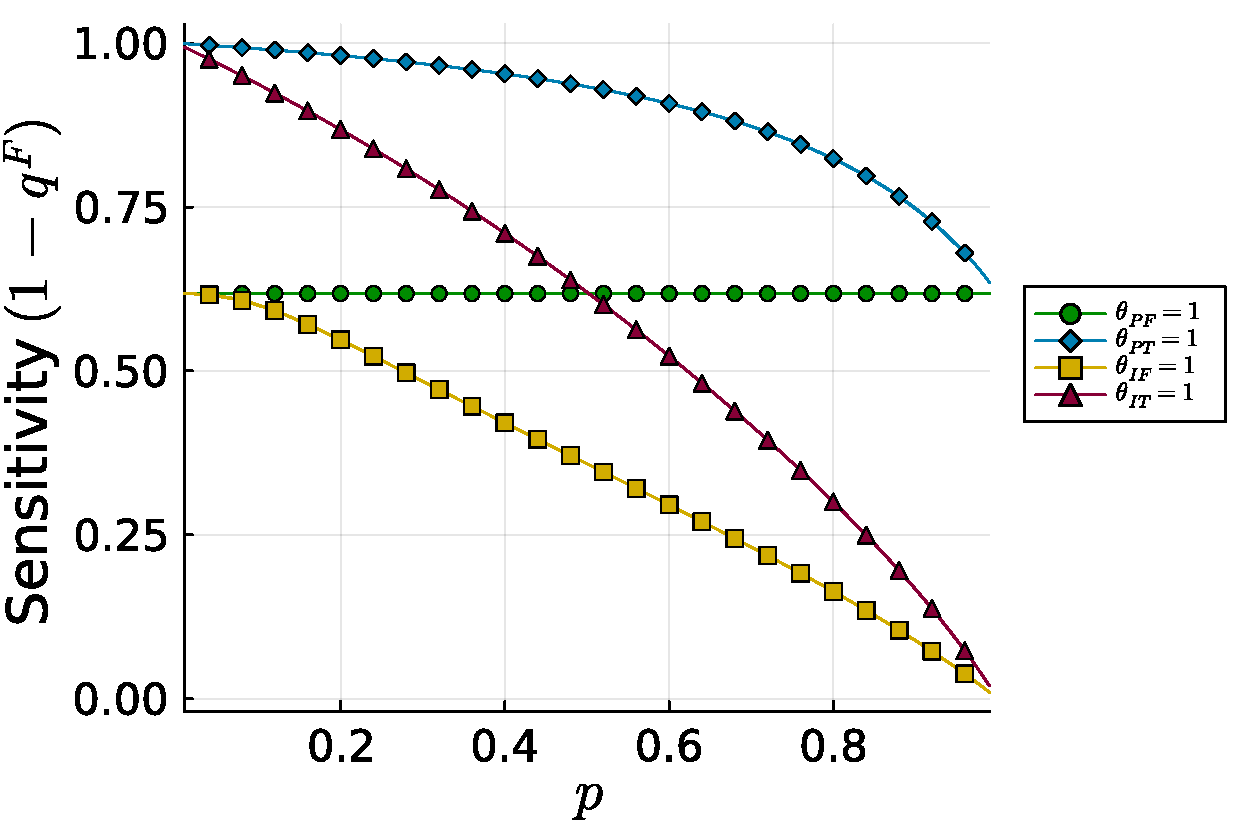
\includegraphics[width = 0.33\textwidth]{Figures/general/genearl_sens.pdf}%
\hspace{0.08\textwidth}%
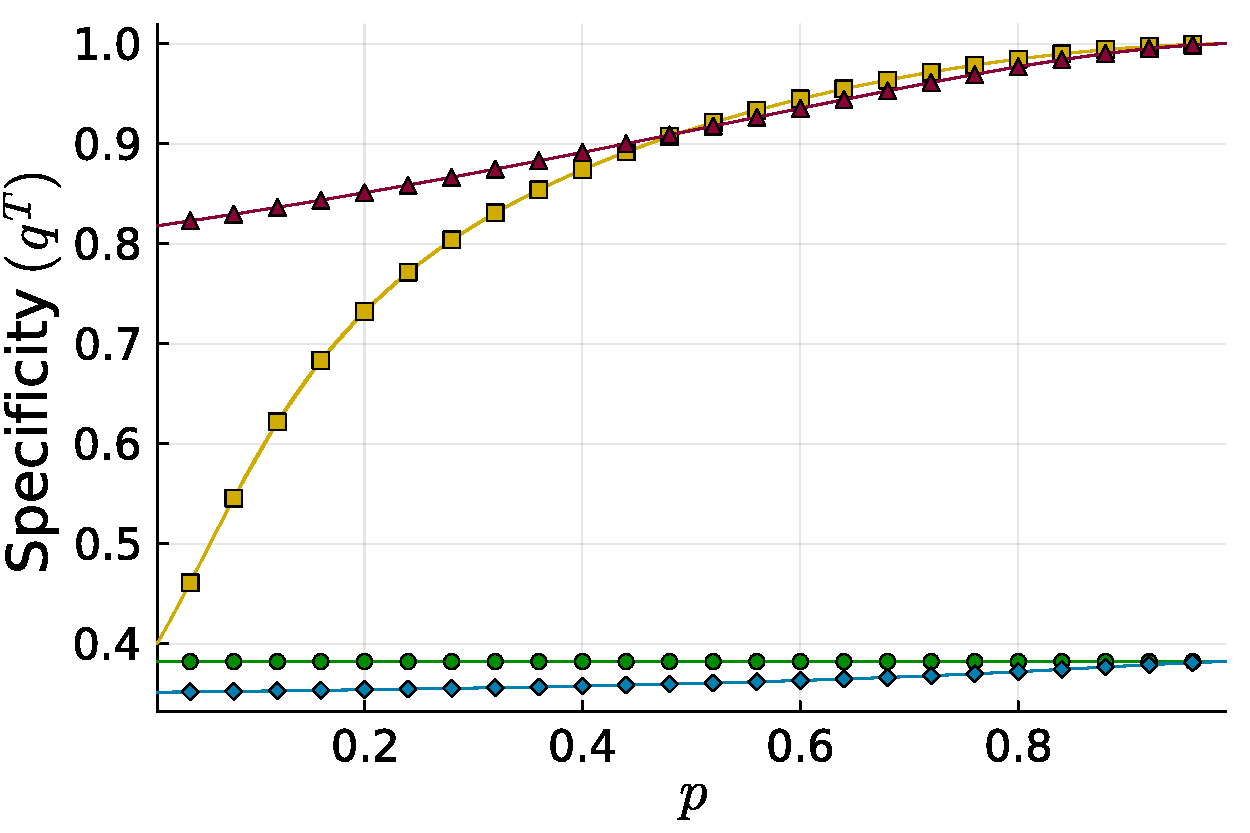
\includegraphics[width = 0.33\textwidth]{Figures/general/general_specificity.pdf}
\\{\small(a)} \hspace{0.45\textwidth} {\small(b)}
\end{tabular}
\caption{(a) Sensitivity and (b) Specificity in the boom equilibrium as a function of the average veracity $p$ of new content for different populations. The meaning of each line is as follows: blue diamonds represent $\theta_{PT}=1$, purple triangles are $\theta_{IT}=1$, green circles are $\theta_{PF}=1$, yellow squares are $\theta_{IF}=1$.  }\label{fig:general_sen_spec}
\end{figure}


Fig.~\ref{fig:general_vol_engage} (a) shows the equilibrium $\delta$ vs $p$, Fig.~\ref{fig:general_vol_engage} (b) shows engagement vs $p$, and Fig.~\ref{fig:general_vol_engage} (c) shows volume vs $p$ for various population types. The population with pure impartial fabulists $(\IF)$ performs no peer filtering as these users do not base their sharing decisions on the truthfulness of the content. This is the same reason why the volume and the engagement are unaffected by changes in the veracity of content. When all users are truthtellers  we see that the equilibrium $\delta$ is high which means that of all viral content, the proportion of true content is high. One interesting observation is that the population with purely partisan truthtellers $(\PT)$ is more effective in peer filtering than even the population with purely  impartial truthtellers $(\IT)$. The reason for this is that the partisan aspect makes it less likely that a user chooses to share any particular content but this decreased sharing reduces the probability of false content going viral more than it does true content. The cost of this higher filtering plays out in Figs~\ref{fig:general_vol_engage} (b) and (c) where purely impartial truthtellers see more volume and more engagement. The population with purely impartial fabulists $(\IF)$, who are the most willing to share content, does a poor job of peer filtering, but the resulting equilibrium has high volume and engagement. Curiously, engagement with purely impartial truthtellers is high even for moderate values of $p$ which is due to the high value of $\delta$ in equilibrium, leading to high likelihood of the content being shared. 

% \begin{figure}[htbp]
% \centering
%     \begin{tabular}{ccc}
%     %\begin{tabular}
% 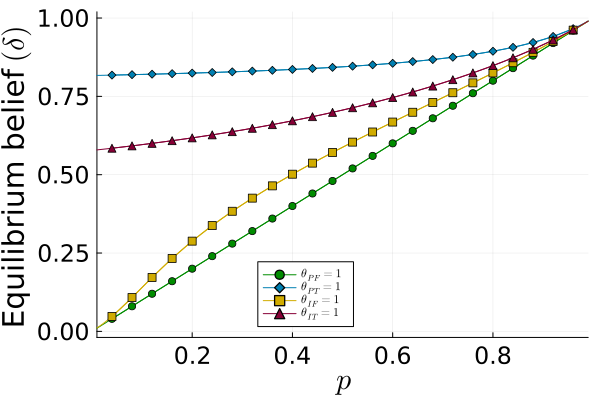
\includegraphics[width = 0.33\textwidth]{Figures/general/general_pd.png}
% 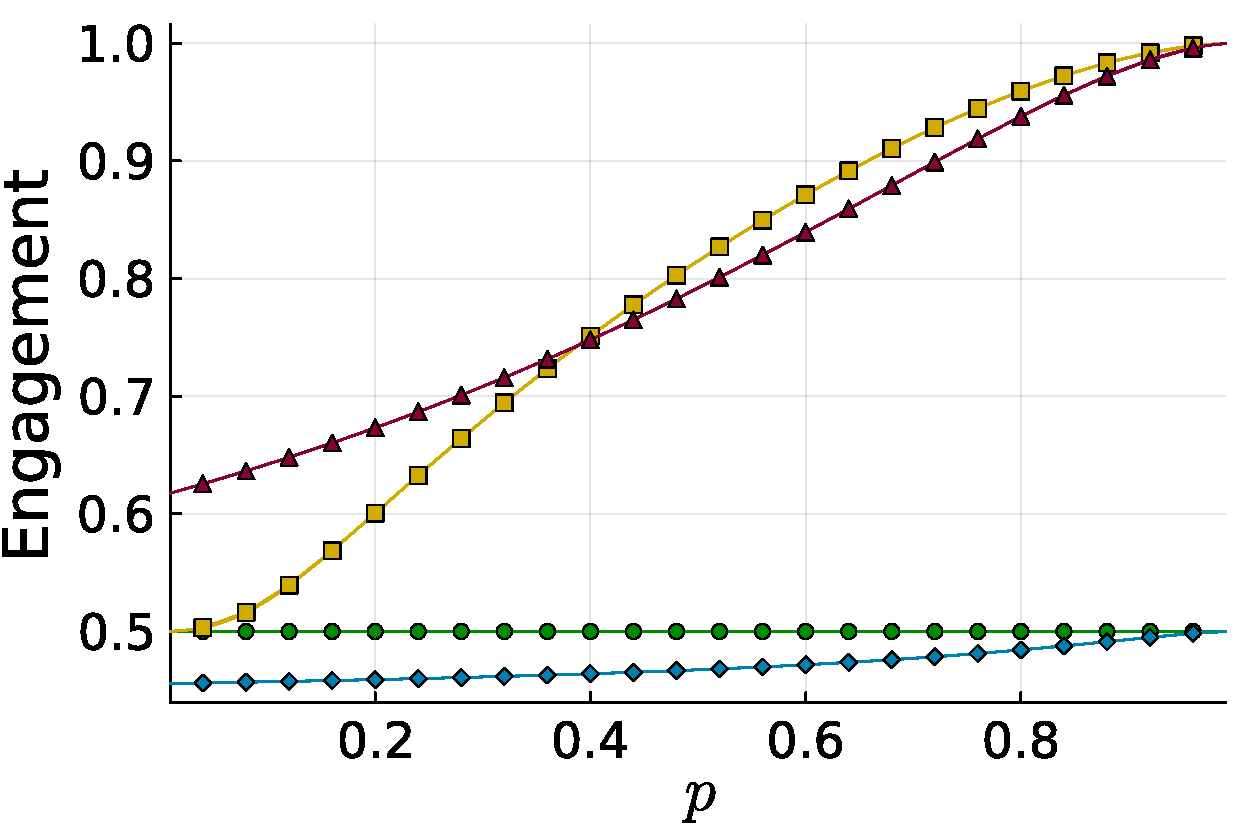
\includegraphics[width = 0.33\textwidth]{Figures/general/general_engage.pdf}
% 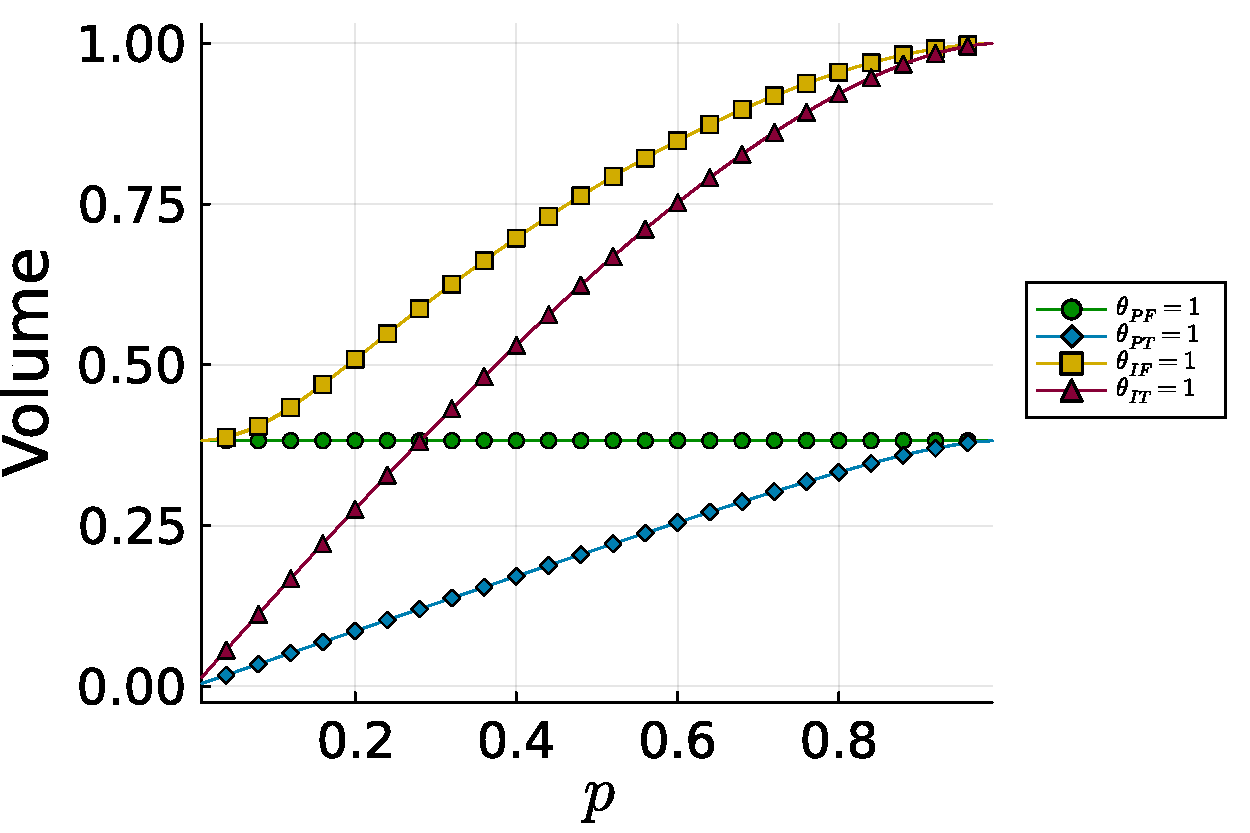
\includegraphics[width = 0.33\textwidth]{Figures/general/general_volume.pdf} \\
% {\small\left(a\right\right) \hspace{{0.25\textwidth}}
% {\small(b\right) \hspace{0.25\textwidth} {\small(c\right)
% \end{tabular}
% \caption\left(a) Average veracity of viral content $\delta$, (b) Engagement level, and (c) volume of viral content as a function p and the population types. The meaning of each line is as follows: blue diamonds represents $\theta_{\PT}=1$, purple triangles are $\theta_{\IT}=1$, green circles are $\theta_{\PF}=1$, yellow squares are $\theta_{\IF}=1$. }\label{fig:general_vol_engage}

% \end{figure}





\section{Conclusions}\label{sec:Conclusions}
We investigated a democratic method for content moderation that uses the wisdom of crowds and the judgment of users in social networks to filter out false information coming into the network. Through the analysis of a simple yet rich model of users in a social network forming beliefs about content veracity and making decisions about sharing the content with their peers, we demonstrated the emergence of the peer filtering phenomenon that leads to higher odds of encountering true information in the network than outside the network. We quantified this phenomenon using metrics including sensitivity, specificity and effectiveness. We further studied the impact of user composition, average content veracity, and platform policies on the level of peer filtering as well as user engagement and content volume in the social network. Our results establish the potential of peer filtering to be a natural and democratic solution to the problem of misinformation spread in online social networks. Our results also highlight that polarization among users does not necessarily increase the level of misinformation. On the contrary, we provided an example in which a more polarized population can have higher peer filtering effect and lower levels of misinformation in the network than a less polarized population.
